% !TeX encoding = UTF-8

% 载入 SJTUThesis 模版
\documentclass[type=master]{sjtuthesis}
% 选项
%   type=[doctor|master|bachelor],     % 可选(默认:master),论文类型
%   zihao=[-4|5],                      % 可选(默认:-4),正文字号大小
%   lang=[zh|en|de|ja],                % 可选(默认:zh),论文的主要语言
%   review,                            % 可选(默认:关闭),盲审模式
%   [twoside|oneside],                 % 可选(默认:twoside),双页或单页边距模式
%   [openright|openany],               % 可选(默认:openright),奇数页或任意页开始新章
%   math-style=[ISO|TeX],              % 可选 (默认:ISO),数学符号样式

% 论文基本配置,加载宏包等全局配置
% !TEX root = ./main.tex

\sjtusetup{
  %
  %******************************
  % 注意:
  %   1. 配置里面不要出现空行
  %   2. 不需要的配置信息可以删除
  %******************************
  %
  % 信息录入
  %
  info = {%
    %
    % 标题
    %
    zh / title           = {上海交通大学学位论文},
    en / title           = {Dissertation Submitted to Shanghai Jiao Tong University for the Degree of Master},
    %
    % 标题页标题
    %   可使用“\\”命令手动控制换行
    %
    zh / display-title   = {基于Agent与知识图谱的任务编排与执行工具的设计与实现},
    en / display-title   = {Design and Implementation of Task Orchestration and Execution Tools Based on Knowledge Graphs and LLMs},
    % 关键词
    %
    zh / keywords        = {上海交大, 饮水思源, 爱国荣校},
    en / keywords        = {SJTU, master thesis, XeTeX/LaTeX template},
    %
    % 姓名
    %
    zh / author          = {蔡卓悦},
    en / author          = {Cai Zhuoyue},
    %
    % 指导教师
    %
    zh / supervisor      = {吴刚},
    en / supervisor      = {Wu Gang},
    %
    % 副指导教师
    %
    % zh / assoc-supervisor  = {某某教授},
    % en / assoc-supervisor  = {Prof.\ Uom Uom},
    %
    % 学号
    %
    id              = {122037910055},
    %
    % 学位
    %   除交叉学科门类外,各一级学科按所属学科门类申请学位
    %   专业学位类别按专业名称申请学位
    %   本科生不需要填写
    %
    zh / degree          = {专业学位硕士},
    en / degree          = {Professional Masters' Degree},
    %
    % 专业
    %
    zh / major           = {软件工程},
    en / major           = {Software Engineering},
    %
    % 所属院系
    %
    zh / department      = {软件学院},
    en / department      = {School of Software},
    %
    % 答辩日期
    %   使用 ISO 格式 (yyyy-mm-dd);默认为当前时间
    %
    % date                 = {2023-05-18},
    %
    % 标题页显示日期
    %   覆盖对应标题页的日期显示,原样输出
    %
    % zh / display-date    = {2023 年 5 月},
    %
    % 资助基金
    %
    % zh / fund  = {
    %                {国家 973 项目 (No.\ 2025CB000000)},
    %                {国家自然科学基金 (No.\ 81120250000)},
    %              },
    % en / fund  = {
    %                {National Basic Research Program of China (Grant No.\ 2025CB000000)},
    %                {National Natural Science Foundation of China (Grant No.\ 81120250000)},
    %              },
  },
  %
  % 风格设置
  %
  style = {%
    %
    % 关键词首行悬挂
    %
    % keywords-format = hang,
  },
  %
  % 名称设置
  %
  name = {
    % bib             = {References},
    % ack             = {谢\hspace{\ccwd}辞},
    % achv            = {攻读学位期间完成的论文},
  },
}

% 使用 BibLaTeX 处理参考文献
%   biblatex-gb7714-2015 常用选项
%     gbnamefmt=lowercase     姓名大小写由输入信息确定
%     gbpub=false             禁用出版信息缺失处理
\usepackage[backend=biber,style=gb7714-2015]{biblatex}
% 文献表字体
\renewcommand{\bibfont}{\zihao{5}\setbaselineskip{16bp}}
% 文献表条目间的间距
\setlength{\bibitemsep}{3bp plus 1pt}
% 导入参考文献数据库
\addbibresource{refs.bib}

% 脚注格式
\usepackage[perpage,bottom,hang]{footmisc}

% 定义图片文件目录与扩展名
\graphicspath{{figures/}}
\DeclareGraphicsExtensions{.pdf,.eps,.png,.jpg,.jpeg}

% 确定浮动对象的位置,可以使用 [H],强制将浮动对象放到这里(可能效果很差)
% \usepackage{float}

% 固定宽度的表格
% \usepackage{tabularx}

% 使用三线表:toprule,midrule,bottomrule。
\usepackage{booktabs}

% 表格中支持跨行
\usepackage{multirow}

% 表格中数字按小数点对齐
\usepackage{dcolumn}
\newcolumntype{d}[1]{D{.}{.}{#1}}

% 使用长表格
\usepackage{longtable}

% 附带脚注的表格
\usepackage{threeparttable}

% 附带脚注的长表格
\usepackage{threeparttablex}

% 算法环境宏包
\usepackage[ruled,vlined,linesnumbered]{algorithm2e}
% \usepackage{algorithm, algorithmicx, algpseudocode}

% 代码环境宏包
\usepackage{listings}
\lstdefinestyle{lstStyleCode}{%
  aboveskip         = \medskipamount,
  belowskip         = \medskipamount,
  basicstyle        = \ttfamily\zihao{-5}\setbaselineskip{12bp},
  commentstyle      = \slshape\color{black!60},
  stringstyle       = \color{green!40!black!100},
  keywordstyle      = \bfseries\color{blue!50!black},
  extendedchars     = false,
  upquote           = true,
  tabsize           = 2,
  showstringspaces  = false,
  xleftmargin       = 1em,
  xrightmargin      = 1em,
  breaklines        = false,
  framexleftmargin  = 1em,
  framexrightmargin = 1em,
  backgroundcolor   = \color{gray!10},
  columns           = flexible,
  keepspaces        = true,
  texcl             = true,
  mathescape        = true
}
\lstnewenvironment{codeblock}[1][]{%
  \lstset{style=lstStyleCode,#1}}{}

% 直立体数学符号
\providecommand{\dd}{\mathop{}\!\mathrm{d}}
\providecommand{\ee}{\mathrm{e}}
\providecommand{\ii}{\mathrm{i}}
\providecommand{\jj}{\mathrm{j}}

% 国际单位制宏包
\usepackage{siunitx}

% 定理环境宏包
\usepackage{amsthm}
% \usepackage{ntheorem}

% 绘图宏包
\usepackage{tikz}
\usetikzlibrary{arrows.meta, shapes.geometric}

% 数据图表宏包
\usepackage{pgfplots}
\pgfplotsset{compat=newest}

% 一些文档中用到的 logo
\usepackage{hologo}
\providecommand{\XeTeX}{\hologo{XeTeX}}
\providecommand{\BibLaTeX}{\textsc{Bib}\LaTeX}

% 借用 ltxdoc 里面的几个命令方便写文档
\DeclareRobustCommand\cs[1]{\texttt{\char`\\#1}}
\providecommand\pkg[1]{{\sffamily#1}}

% hyperref 宏包在最后调用
\usepackage{hyperref}

% E-mail
\providecommand{\email}[1]{\href{mailto:#1}{\urlstyle{tt}\nolinkurl{#1}}}


\usepackage{tcolorbox}
\usepackage{xcolor}

\begin{document}

%TC:ignore

% 标题页
\maketitle

% 原创性声明及使用授权书
\copyrightpage
% 插入外置原创性声明及使用授权书
% 此时必须在导言区使用 \usepackage{pdfpages}
% \copyrightpage[scans/sample-copyright.pdf]

% 前置部分
\frontmatter

% 摘要
\input{contents/abstract}

% 目录
\tableofcontents*
% 插图索引
\listoffigures*
% 表格索引
\listoftables*
% 算法索引
\listofalgorithms*

%TC:endignore

% 主体部分
\mainmatter

% 正文内容
% !TEX root = ../main.tex

\chapter{绪论}

\section{研究背景与意义}

居民消费和出行是当前经济社会发展的核心议题之一。《扩大内需战略规划纲要(2022-2035年)》强调,构建完整的内需体系是推动经济高质量发展的必然选择。在此背景下,人工智能技术,作为新一代信息技术的代表,将在促进消费和出行领域的智能化转型中发挥关键作用。

近年来,人工智能在经济发展和社会治理中展现了广泛的应用潜力。《中华人民共和国国民经济和社会发展第十四个五年规划和2035年远景目标纲要》明确提出,未来十年内,人工智能将在关键核心技术方面取得重大突破,推动智能化在各个领域的应用。"十四五"期间提出的三大人工智能发展布局——突破核心技术、打造数字经济新优势、营造良好数字生态——为消费和出行领域的智能化升级奠定了坚实的基础。

随着大语言模型(Large Language Model, LLM)的快速发展,其在消费和出行领域的应用逐渐凸显。大语言模型能够处理海量数据,具备强大的自然语言理解与生成能力,为智能化工具的集成提供了技术支持。通过将LLM与消费、出行等领域的工具集成,能够有效提升用户体验和服务效率。例如,基于大语言模型的智能体可以调用多种消费和出行相关的API,自动识别用户需求,为用户提供个性化的决策支持和出行规划。

在此过程中,知识图谱的角色也发生了显著转变。过去,知识图谱主要用于构建领域内的结构化知识,建立实体及其关系网络,帮助系统实现更加精准的信息检索和问答。它依赖专家手工构建或自动化系统提取的知识,能够为特定领域中的推理提供逻辑支持。知识图谱的强项在于关系推理、知识验证以及为复杂任务提供可解释性。

如今,在大语言模型的语境中,知识图谱不再仅仅是孤立的信息源,而成为大语言模型的重要补充和增强工具。大语言模型具备广泛的语义理解和生成能力,但由于缺乏严格的逻辑结构和推理框架,有时会出现逻辑不连贯或生成内容不够精准的问题。而知识图谱可以弥补这一不足:通过将结构化的知识与大语言模型结合,知识图谱能够为大语言模型提供精准的背景信息与逻辑推理能力。具体而言,在智能体工具利用领域,知识图谱可以帮助大语言模型在复杂任务中识别工具之间的关系,辅助工具调用路径的优化,并增强模型的可解释性和推理能力。

尽管大语言模型在工具调用和集成方面展现了显著的潜力,仍然存在以下关键问题:

\begin{itemize}
    \item 无法集成大规模工具:当前的系统虽然 可以调用多种API,但面对大量的工具集成时,表现出局限性。大语言模型需要处理不同工具的数据格式、调用方式以及响应速度,当工具数量较大时,模型的调用能力和协调效率会明显下降,难以实现对大规模工具的无缝集成。这种限制影响了系统在复杂场景中的适应性与灵活性。
    \item 难以处理工具之间的依赖关系:对于涉及多个工具协同工作的任务,模型在处理工具间的依赖关系时往往力不从心。例如,在消费推荐和出行规划的场景中,某些工具的输出需要成为下一个工具的输入,且各工具的调用顺序和逻辑关系十分重要。目前,大语言模型难以有效管理这些复杂的依赖关系,容易导致任务流程的中断或结果的误差。
\end{itemize}


\section{国内外研究现状}
本节将会概述针对大语言模型智能体和知识图谱的研究进展。首先,本节会介绍大语言模型智能体工具调用方面的研究,分为基于提示词工程的方法和基于模型微调的方法。其次,本节将聚焦于大语言模型规划、推理提升的方面,包括提示词工程和模型微调的方法。最后,本节还会介绍知识图谱和大语言模型结合的应用,比如如何利用知识图谱中的外部知识增强大语言模型,以及如何在图谱上进行推理。

\subsection{大语言模型智能体工具调用}

外部工具的引入不仅能够增强大语言模型的能力,比如获取最新知识、提升专业技能,流程自动化、交互增强等。同时,外部工具的采用也能够提高生成过程中的透明性和鲁棒性,让回答更加可靠和可解释。在大语言模型智能体工具调用领域,研究人员已经提出了许多方法来实现大语言模型工具调用。总体来讲,许多工作中的大语言模型工具调用流程都包含以下四个阶段:任务规划、工具选择、工具调用和响应生成\cite{Ruan2023, Shen2023, Song2023}。

本文主要聚焦于任务规划和工具选择的部分,即如何根据用户需求从众多工具中选择合适的一个或一组工具来形成工具调用链来完成用户的需求。

\subsubsection{工具任务规划}
在现实的信息查询场景中,用户的查询需求往往包含复杂的意图,如何识别用户意图是工具调用的首要问题。因此在工具任务规划阶段,我们首先需要将用户的需求语句转化为更加明确的任务,进行子任务的拆解和任务之间的关联分析。任务规划方式一般分为基于提示词工程的方式和基于微调的方式。

\paragraph{基于提示词工程的工具规划} 
现有研究\cite{Miao2023}表示,大语言模型能够通过少样本甚至零样本实现有效的任务规划。HuggingGPT\cite{Shen2023}首先把任务分解为各种子任务,然后选择合适的模型来解决这些子任务。RestGPT\cite{Song2023}引入了一种从粗粒度到细粒度的规划方法,能够指导大语言模型逐步对任务进行分解。ControlLLM\cite{Liu2023a}引入了一种叫做“在图上思考”(Think-on-graph, ToG)的范式,通过深度优先搜索算法(DFS)在构建好的工具图上进行搜索,得到解决方案。

\paragraph{基于微调的工具规划} 

Toolformer通过工具调用来辅助模型预测后续词元,基于此原理对模型进行了微调,从而提升大语言模型的工具认知和工具调用效率。TookenGPT中将工具作为了特殊词符,以生成普通文字输出的方式对外部工具进行调用。α-Umi提出了一种新的两阶段的训练模式,首先对基础大语言模型进行较为通用的微调,随后细分为规划器、调用器等模块,分别进行更加针对性的微调。

\subsubsection{工具选择}
在任务规划阶段完成后,需要根据每个子任务进行工具选择。工具选择过程一般有两种途径:一种是通过训练得到的检索器来选择工具,另一种是直接让大语言模型从工具列表中选择合适的工具。

\paragraph{基于检索器的工具选择} 
当工具数量过多时,通常会使用检索器先搜索得到与任务相关的工具。检索方式包括基于关键词的检索和基于语义的检索两种。

\begin{enumerate}
    \item \textbf{基于关键词的检索}:如TF-IDF\cite{Jones1972}和BM25\cite{Robertson2009}。这些方法通过精确匹配实现用户需求和文档之间的对齐和查询。
    \item \textbf{基于语义的检索}:利用神经网络来学习文本之间的语义关系,然后使用余弦相似度等算法计算语义相似度,如ToolLLM\cite{Qin2023}。
\end{enumerate}

\paragraph{基于大语言模型的工具选择} 

在工具数量有限,或者是已经检索得到少量有关工具时,可以让大语言模型利用自身的推理和分析能力选择最合适的工具。具体来说,我们可以将备选工具的工具名称、工具描述信息和参数列表与用户需求一起放入大语言模型的输入上下文,提供给模型。随后,模型根据用户需求选择合适的工具。现有的基于大语言模型的工具调用方法分为两类:基于提示词工程的方法和基于模型微调的方法。

\textbf{基于提示词工程的方法}:该方法利用大语言模型的上下文学习能力,通过编写提示词来进行工作。有一些通用的提示词技巧可以帮助在多个工具中选择正确的工具。Chain of Thought(CoT)\cite{Wang2023a}在提示词中加入了例子,让大模型在解决复杂问题时采取相应的推理步骤,让大模型以分步的方式来规划和行动。Re-Prompting\cite{Raman2022}在生成计划之前会检查每个步骤是否能够执行。如果不能够执行,则让大模型重新生成计划。Self-consistent CoT(CoT-SC)\cite{}因此让大模型执行多条推理路径,选择出现频率最高的答案输出。Tree of Thoughts(ToT)\cite{Yao2023a}用树状的形式组织推理过程,树上的每个节点表示一个“想法”即推理中间步骤。中间步骤的选择基于大模型的评估,最终计划用深度优先遍历(DFS)或者广度优先遍历(BFS)得出。在GoT\cite{Besta2023}中,作者把用树状结构组织推理扩展为了用图结构组织。

引入环境反馈同样可以提升能力,ReAct\cite{Yao2023b}中指导大模型按照thought-action-observation的方式来解决问题。生成的想法来帮助大模型进行推理和规划,基于这个想法大模型会采取不同的行动,最后观察该行为的结果并作为反馈提供给大模型。Voyager\cite{Wang2023b}里智能体接收的反馈包括三种:程序执行的中间结果、执行错误描述和自我验证结果。Inner Monologue\cite{Huang2022}主动获取人类的反馈,将其与环境反馈进行结合,用于增强大模型的规划和推理能力。SelfCheck\cite{Miao2023}则让智能体对自己的推理步骤进行检查和评估,根据结果来修改计划以提升性能。

关于专门针对工具选择场景的提示词工程和流程搭建工作,ToolNet\cite{Liu2024}将大量工具组织成为有向图的形式,允许大语言模型从初始节点出发,迭代地在图上选择下一个工具,直到完成任务。ToolLLM\cite{Qin2023}中提出了基于深度优先遍历算法的决策树算法,通过支持回溯操作解决了在工具选择上的错误传播问题,有效提高了整体的准确性和通过率。AnyTool\cite{Du2024}提出了一种自我反思的层次化选择的方法,通过在结构化的工具调用树上迭代选择合适的工具。

\textbf{基于模型微调的方法}:该方法通过对大语言模型进行参数微调,以提高其在工具选择中的表现。此类方法通常涉及到利用额外的训练参数或者针对性训练,从而增强模型的工具选择能力。ToolLLaMA\cite{Qin2023}利用在ToolBench数据集中DFSDT算法所得到的的指令-推理轨迹对微调了LLaMA-7B的模型,有效增强了开源大模型的工具能力。ToolAlpaca\cite{Tang2023}提出了一种自动化构建工具调用数据的框架,构建了3.9K条工具调用数据集微调得到了ToolAlpaca-7B和ToolAlpaca-13B的模型。ToolVerifier\cite{Mekala2024}提出了一种“自我验证”的思想,通过在工具选择过程中自问自答一组问题来区分相似的候选工具。
不管是基于提示词工程还是基于模型微调的方法,都有各自的优缺点和特点,但是都能够有效提升模型的工具选择能力。基于提示词工程的方法不需要对模型参数进行修改,通过精心构建的提示词构建和流程搭建来提升大语言模型在工具选择中的能力,并适用于所有的大语言模型。而基于模型微调的方法相对复杂,并且仅能适用于开源大语言模型。在微调中需要消耗计算资源,通过调整参数的方式将工具有关的知识注入到模型中。

\subsection{大语言模型与知识图谱结合的应用}

尽管大语言模型主要用于纯文本的场景,但是在许多现实场景中,文本数据与丰富的结构信息以图谱的方式存储。此外,大语言模型的基于文本的推理能力已经得到较多的展现,但是大语言模型在图谱上的推理能力仍有很大的探索空间。

通过将现实世界的知识表示为结构化的知识图谱,并在图谱上进行推理和演算,能够解决许多重要问题。

关于如何将图谱上的知识提供给大语言模型的问题,有三种常见的方法:

\begin{enumerate}
    \item 自然语言描述。用自然语言描述图结构是最简单的方式,可以直接描述图上的边和邻接列表。
    \item 对图进行文本上的改写。由于自然语言描述图通常会较为复杂,而且不具备结构化的特点,因此对图的描述进行了改写,得到了更加高效的图的描述,有利于模型对图谱信息的利用。
    \item 对图进行编码。最后一种方法是通过训练图编码器,将图结构编码成为特征序列并作为特征的一部分输入到大语言模型中。这种方法涉及到对大语言模型的微调,以让其适应新的输入格式。
\end{enumerate}

通过将图谱的信息通过自然语言文本或者嵌入向量的格式输入到大语言模型上,可以在图谱上进行推理和搜索。常见的做法是利用深度优先搜索算法(DFS)或者广度优先搜索算法(BFS)来实现在图上的推理和搜索。许多研究探索了基于搜索的推理,特别是在知识图谱领域。Reasoning on Graph\cite{Luo2023}的方法将知识图谱作为可靠的知识来源,通过提示大语言模型生成多个关系路径作为计划,随后根据这些路径不断在知识图谱上搜索,有效地提高了回答的可信度和效率。另一种方法是在图谱上动态地进行迭代检索和推理子图来模拟动态搜索过程\cite{Liu2024, Sun2023, Ma2024}。在每个步骤中,大语言模型都检索当前节点的邻居节点,然后决定下一步操作是继续搜索还是结束搜索并给出答案。在ToolNet\cite{Liu2024}中,作者根据工具调用的数据集建立了图谱,并根据图谱上的边进行搜索,迭代式选择所需的工具进行调用,有效提升了工具搜索的准确性。Think-on-Graph系列\cite{Sun2023,Ma2024}在知识图谱上通过大语言模型Agent进行迭代式的束搜索,探索发现最好的推理路径,并返回最有可能的推理结果。

这些方法的优点在于,通过图谱的辅助,系统不仅能够提供对应的答案,还可以提供图谱片段作为可以解释的证据。同时,由于知识图谱存储的数据量可以扩展,这些方法通过在图上搜索也增加了系统的可扩展性。

\section{研究问题}

基于以上的研究背景,本文的核心研究问题归纳如下:
\begin{itemize}
    \item \textbf{如何通过工具调用轨迹数据构建一个高效且结构化的工具知识图谱?}
   本问题旨在研究如何筛选、清洗现有的工具调用轨迹数据,并构建一个大型工具知识图谱,从而将轨迹中的工具知识有效地嵌入到图谱中。重点探讨数据清洗的标准和方法、知识图谱构建的技术路径,以及如何使该图谱在后续的工具搜索和优化流程中发挥有效作用。
    \item \textbf{如何结合知识图谱与智能体架构实现自动化工具编排和调用?}
   本问题关注如何基于知识图谱和智能体架构,设计一个完整的任务分解、工具选择、调用以及结果解析的流程框架。研究重点包括:智能体如何高效利用知识图谱进行工具调用路径的优化,如何在真实API环境下验证智能体编排的有效性,以及如何提升工具调用的精确性和任务完成效率。
\end{itemize}

\section{研究内容}
本文主要研究基于Agent与图谱的任务编排工具的设计与实现流程,主要针对用户进行信息查询时的便利。本文研究与实现的内容主要包括以下几点:

\begin{enumerate}
    \item 本文提出了一种基于工具调用轨迹数据构建大型工具知识图谱的方法,旨在辅助智能工具搜索与调用流程。首先,通过两种数据筛选策略,筛选出高质量的API工具轨迹数据。接着,设计了工具点权和边权值的计算方法和动态更新方法,以表示工具之间的转换关系和工具可用性。最后,通过对比包含图谱知识与传统检索增强方式,验证了工具知识图谱在实际应用中的有效性。
    \item 为了有效利用构建的工具知识图谱的知识,本文提出了基于DFS的工具动态搜索算法。该方法通过在图谱上进行深度优先搜索和动态回溯,能够充分利用图谱上的知识选择工具路径。同时,我们提出了长短期记忆框架,通过维护长短期记忆知识,进一步辅助大语言模型的规划和推理。通过在真实世界的API测试集上进行实验,验证了该方法的有效性,并且证明该方法优于基线方法。
    \item 本文设计并实现了一个基于知识图谱和大语言模型的智能API编排与调用系统,旨在提供用户友好的交互体验。本工作允许用户通过自然语言提问,系统能够解析需求并自动调用相关API,生成答案。其主要功能包括用户登录、API调用流程可视化、问答服务以及自定义工具添加,而管理员可以管理模型超参数配置和数据库。系统的整体架构分为存储层、访问层、功能层、接口层和展示层五层,各层负责不同的功能,以确保系统的高效性和易用性。
\end{enumerate}

\section{论文组织结构}

本论文的内容组织结构分为以下几章:

\indent 第一章为绪论,本章节从研究背景出发,依次介绍了本文研究的问题以及难点,国内外的研究现状,以及本文的主要工作内容以及本文组织结构。

\indent 第二章为相关理论与技术,本章主要介绍了有关的一些概念以及现有的技术方案等。首先介绍了知识图谱的概念以及分类,基于API知识图谱的研究。其次介绍了大语言模型的定义、发展历史以及大语言模型有关的技术:大模型智能体、提示词工程、检索增强技术等。最后,本章介绍了有关大语言模型和知识图谱结合的应用方案。

\indent 第三章为基于工具调用轨迹的知识图谱构建方法及实现。本章主要介绍了如何针对现有的工具调用轨迹数据进行筛选和清洗,并根据其构建一个大型的工具知识图谱。通过边权和点权的更新来表示工具知识,以辅助后续的工具搜索流程。

\indent 第四章为基于知识图谱和智能体的工具编排和调用方法的设计与实现。本章聚焦于大模型工具任务的各阶段,比如如何完成任务分解、工具选择、工具调用、结果解析等流程。并在真实世界的API工具上设计测试集验证了该方法的有效性。

\indent 第五章为系统设计和实现。对系统的架构以及各功能模块进行了设计与实现,在实现前几章各模块的基础上实现了可视化界面和流程搭建。具体内容包括有系统框架设计,系统功能模块介绍以及系统展示等。

\indent 第六章为总结与展望,对全文的研究工作进行了回顾,总结了成果,并且对本研究的局限性和未来的研究方向进行了展望。
% !TEX root = ../main.tex

\chapter{相关技术分析}

\section{传统服务编排}

随着互联网技术的快速发展,用户对软件系统需求日益增加。为平衡服务稳定性和需求灵活性,微服务架构应运而生。相比于面向服务的体系架构(Service Oriented Architecture,SOA),微服务架构更注重服务的独立性。每个微服务作为独立单元开发、部署、扩展,通过定义明确的接口提供服务。这种架构大幅提升了软件系统的灵活性与可扩展性。

\subsection{服务编排模式}
在微服务架构中,多个服务协作完成完整业务流程的过程称为服务编排。常见的编排方式有两种:
\begin{itemize}
    \item \textbf{服务编制}:中心化模式,控制中心定义服务的执行流程,各服务无需了解具体组合顺序。
    \begin{figure}[h]
        \centering
        \begin{tikzpicture}[node distance=2cm]
            % Nodes
            \node[draw, circle] (control) {控制中心};
            \node[draw, rectangle, below left of=control] (service1) {服务 1};
            \node[draw, rectangle, below of=control] (service2) {服务 2};
            \node[draw, rectangle, below right of=control] (service3) {服务 3};
            % Arrows
            \draw[->] (control) -- (service1);
            \draw[->] (control) -- (service2);
            \draw[->] (control) -- (service3);
        \end{tikzpicture}
        \bicaption{服务编制模型}{Service Compositon}
        \label{fig:service-composition}
    \end{figure}

    \item \textbf{服务编排}:去中心化模式,服务通过消息队列等机制相互通信,完成资源与信息的交换。
    \begin{figure}[h]
        \centering
        \begin{tikzpicture}[node distance=2cm]
            % Nodes
            \node[draw, rectangle] (service1) {服务 1};
            \node[draw, rectangle, right of=service1] (service2) {服务 2};
            \node[draw, rectangle, right of=service2] (service3) {服务 3};
            \node[draw, rectangle, below of=service2] (queue) {消息队列};
            % Arrows
            \draw[->] (service1) -- (queue);
            \draw[->] (queue) -- (service2);
            \draw[->] (service2) -- (queue);
            \draw[->] (queue) -- (service3);
        \end{tikzpicture}
        \bicaption{服务编排模型}{Service Orchestration}
        \label{fig:service-orchestration}
    \end{figure}
\end{itemize}

两种方式都旨在组合与协调微服务,提供复杂业务支持。

\subsection{服务编排实现方式}
微服务架构提出后,涌现了许多编排工具与语言,例如 BPEL 和 BPMN。
\begin{itemize}
    \item \textbf{BPEL}(Business Process Execution Language):基于 XML 的标准服务编制语言,用于定义业务流程的抽象和可执行方案。
    \item \textbf{BPMN}(Business Process Model and Notation):业务流程建模语言,简化了流程设计与实施的沟通,适合流程可视化建模。
\end{itemize}

此外,Netflix Conductor、Zeebe 等流程引擎,以及 Activiti、jBPM 等开源框架,提供了更多编排支持。实际应用中,许多项目采用 BPMN 或 BPEL 结合工作流框架构建微服务系统。

然而,传统方法面临以下挑战:
\begin{enumerate}
    \item \textbf{复杂性与适应性}:如 BPEL 需清晰接口定义,但许多现实 API 接口不规范,若要转为规范定义需人工参与。
    \item \textbf{快速迭代的需求}:由于持续集成等概念的流行,服务编排不仅需要能够静态地组合定义规范的服务,还需要支持快速组合新加入的服务。
    \item \textbf{高门槛与资源消耗}:对于众多且不断变化的业务需求,每次都需要开发人员全程参与,对微服务进行明确定义、对业务流程重新进行编排,需要耗费大量人力。
\end{enumerate}

本项目通过结合大语言模型(LLM)的语义解析能力与知识图谱技术,提出低门槛的服务编排方案。利用 LLM 对用户需求自动解析,结合知识图谱自动生成服务调用流程,减少开发者参与和人力成本。最终目标是实现用户需求驱动的智能化服务编排,提升效率与灵活性,同时降低学习和部署成本。

\section{知识图谱}

\subsection{知识图谱的简介与定义}

知识图谱是一种对现实世界中知识和概念进行建模的技术。虽然“知识图谱”这一术语早在1972年便已出现\cite{schneider1973course},但现代意义上的知识图谱概念起源于谷歌在2012年发布的 Google Knowledge Graph\cite{singhal2012knowledge,zou2020survey}。
知识图谱采用基于图的数据模型,适用于需要整合、管理和从多样化的数据中提取价值的应用场景\cite{noy2019industry}。
最初,知识图谱旨在增强搜索引擎的理解能力,为用户提供更加智能化的搜索体验。
然而,随着技术的不断发展,知识图谱如今已被广泛应用于人工智能领域,包括语义搜索、推荐系统、大数据分析、智能问答系统等。

在知识图谱中,知识以结构化图的形式表示,其中节点用于表示实体,如人物、地点、事件或抽象概念,
而节点之间的边则表示实体间的语义关系或逻辑关联。
知识图谱的核心单元是三元组 (subject, predicate, object),
即“头实体-关系-尾实体”。
这种形式化的表达方式使得知识可以在不同系统中共享、分析和推理,为各类人工智能应用提供支持。

\vspace{0.5em}

知识图谱可以形式化地定义为一个有向图 $G = (V, E, R)$,其中:
\begin{itemize}
    \item $V$ 是节点集合,表示知识图谱中的实体或概念;
    \item $E \subseteq V \times R \times V$ 是边集合,表示实体之间的关系;
    \item $R$ 是关系集合,定义了节点之间可能的语义或逻辑关系。
\end{itemize}

每条边 $(h, r, t) \in E$ 表示一个三元组,其中:
\begin{itemize}
    \item $h \in V$ 是头实体(head entity);
    \item $r \in R$ 是实体之间的关系(relation);
    \item $t \in V$ 是尾实体(tail entity)。
\end{itemize}

通过这种结构化的三元组表示,知识图谱能够捕获实体及其相互间的复杂关系,支持语义推理、知识查询和知识增强等应用。

\subsection{知识图谱的种类}
知识图谱的发展大致经历了四个阶段\cite{Jiang2023}:

\begin{enumerate}
  \item \textbf{静态知识图谱}: 早期的知识图谱大多都用于存储静态知识,其中的三元组不被更新或不常被更新。
  \item \textbf{动态知识图谱}: 为了保证知识的实时性,知识图谱需要定期被修改或更新。
  \item \textbf{时序知识图谱}: 时序知识图谱中加入了时序信息的表示,能够提供一种更全面的在时序上了解知识的方式。
  \item \textbf{事件知识图谱}: 事件知识图谱的重点在于如何表示和理解事件。事件会涉及不同的实体和关系,而且在特定的时间段发生,这让事件表达变得格外困难。事件知识图谱对图谱的结构进行了修改,加入了表示事件的节点和两种不同的关系形式(实体-事件关系和事件-事件关系)。
\end{enumerate}

\subsection{知识图谱的应用}



\section{大语言模型}

\subsection{大语言模型的定义}

大语言模型(LLMs)主要指基于Transformer架构的语言模型,
通常具有数十亿到百亿个参数。
LLM通过在海量文本数据上进行预训练,
学习词汇、句法、语义和语境之间的关系,
能够生成和理解复杂的自然语言。
形式化定义如下:

设有一个语言模型 \( \mathcal{M} \),它通过给定一个输入序列 \( x = (x_1, x_2, \dots, x_n) \) 来预测下一个词或生成输出序列 \( y = (y_1, y_2, \dots, y_m) \)。模型的目标是最大化给定上下文时生成词的联合概率分布 \( P(y_1, y_2, \dots, y_m | x_1, x_2, \dots, x_n) \)。这个联合概率可以通过链式法则表示为:

\[
P(y_1, y_2, \dots, y_m | x_1, x_2, \dots, x_n) = \prod_{i=1}^{m} P(y_i | y_1, \dots, y_{i-1}, x_1, x_2, \dots, x_n)
\]

其中,\( P(y_i | y_1, \dots, y_{i-1}, x_1, x_2, \dots, x_n) \) 是模型在给定先前上下文和输入序列时对 \( y_i \) 的条件概率预测。

随着大语言模型参数量和规模的提升、
以及训练文本量的增大,大语言模型展现出了小模型不具有的“涌现能力”。
比如:(1)上下文学习能力,大语言模型能够从提示词中提供的小规模样本中学习如何完成新任务。
(2)指令遵循能力,在经过指令微调后,大语言模型能够遵循新任务的指令。
(3)复杂推理能力,大语言模型能够通过将复杂任务分解为中间推理步骤来解决复杂任务。
大语言模型还可以通过外部知识和工具调用来增强,以便获得更强大的能力和提升任务的准确性和可靠性。

现有的大模型根据是否开源可以分为两种,第一种是闭源的商业大模型,如:GPT系列\cite{achiam2023gpt, OpenAI2023},Claude系列\cite{anthropic2023claude3},Gemini\cite{team2023gemini, team2024gemini}等等,
这些模型的权重不开放给开发者,因此只能通过官方提供的平台或者API接口来使用这些模型;
另一种是开源的大模型,比如:Baichuan\cite{Yang2023},ChatGLM\cite{Zeng2023},
Qwen\cite{yang2024qwen2},LLaMA\cite{Touvron2023}等。
这类模型的效果一般比商业大模型的效果弱一些,但由于是开源的,开发者可以根据具体需求构建数据集对模型有监督的微调等进一步参数调整,也可以部署在本地GPU服务器上。

\subsection{大语言模型提示词工程}

提示词工程是通过创建自然语言指令(Prompt)来从大语言模型中提取知识的过程,已成为提升预训练大语言模型能力的重要技术之一。通过精心设计提示词,可以在不更改模型参数的情况下提高模型输出的表现。与传统方法相比,提示词工程无需对模型进行训练或微调即可实现特定任务上的性能提升,从而有效增强大语言模型在不同领域的适应性和可用性。

目前提示词工程的技术体系十分多样化,涵盖了从最基本的零样本提示(Zero-Shot Prompting)和少样本提示(Few-Shot Prompting)到更复杂的“思维链提示”(Chain of Thought Prompting)等多种方法。
我们可以根据是否提供自然语言文本的参考样本将提示词方法分为以下两种。

\begin{itemize}
    \item \textbf{零样本提示(Zero-Shot Prompting)}:在零样本提示设置(Zero-Shot,Radford等,2019)中,大语言模型完全依赖于在预训练过程中学到的知识,通过提示词中的指令直接执行任务,而无需任何额外的示例数据。该方法的优点在于操作简单,但在任务理解和推理复杂度上往往会受到限制。
    \item \textbf{少样本提示(Few-Shot Prompting)}:在少样本提示设置中(Few-Shot,Brown等,2020),为了更好地理解任务,除了提供任务指令,还会加入少量的示例数据点来帮助模型掌握上下文语境和任务要求。研究表明,精心设计的少样本提示能够显著提升模型的性能,但如果选取的示例不当,模型可能会对这些样本产生难以预料的偏差。少样本提示策略在提示词工程中被视为一种有效的方式,用于提升模型的规划和推理能力。
\end{itemize}

除了根据提示词中的样本数量分类,许多提示词会规定大语言模型用特定的模式来进行,以下是几种针对提升大语言模型在复杂推理任务中的能力而提出的提示策略:

\begin{itemize}
    \item \textbf{基本提示(Basic/Vanilla Prompting)}:基本提示是最基础和最简单的提示词策略,指的是直接向语言模型提供任务,而不进行任何提示词策略的优化。该方法的目标是评估模型在没有提供外部信息时的性能表现。在不同的研究中,基本提示也被称为“标准提示”或“原始提示”,常作为各类提示策略的基础对比。
    \item \textbf{思维链提示(Chain-of-Thought,CoT)}:\cite{Wang2023a}提出了一种思维链提示策略,该策略通过将复杂问题分解为更容易理解的子问题,然后逐步推理并整合各个子问题的解答来得出最终答案。这种方法模拟了人类在解决问题时的逐步推理过程,展示了显式推理链条对复杂任务的性能提升效果。
    \item \textbf{思维树提示(Tree-of-Thought,ToT)}:该提示词框架在思维链的基础上进行扩展,以树状结构管理中间推理步骤,进一步增强了大语言模型在面对复杂任务时的推理能力。思维树结合了模型生成和评估“思维”的能力,并使用了一些常见的搜索算法,如深度优先算法和广度优先算法来在树上进行搜索。在思维树框架下,模型可以系统化地对不同推理路径进行探索,并且在出现错误时能够及时回溯。
    \item \textbf{自我一致性提示(Self-Consistency)}:自我一致性提示通过生成多个回答并选择出现频率最高的答案来提高思维链的表现,有利于提升推理的准确性和一致性。
    \item \textbf{ReAct提示词}:该策略通过将复杂问题分解为更容易理解的子问题,然后逐步推理并整合各个子问题的解答来得出最终答案。在每一步,系统都会生成思维(Thought)、行为(Action)和观察(Observation)三部分的内容,并加入大语言模型的上下文来提示模型进行推理。
\end{itemize}

\subsection{大语言模型智能体}

大语言模型也可以作为“Agent”来为用户提供服务。智能体的概念的最早可以追溯到古希腊时期的哲学家亚里士多德和休谟等人\cite{Zalta2019}。从大体上来讲,智能体可以被定义为“含有欲望、信念、动机和行为能力的实体”\cite{Xi2023}。后来,计算机科学中也用到了智能体这个概念,在人工智能领域中的AI智能体就用来描述具有自主性、主动性、反应性和智能行为能力的实体\cite{Wooldridge1995}。
早期的AI智能体研究主要集中在增强智能体的特定能力上\cite{Sutton2018},并通过改进相应算法和训练策略来提升它们的表现,而忽略了模型本身如记忆、推理能力的综合能力的提升。
然而,模型本身的能力很大程度上决定了智能体在任务上的表现。

近年来,随着大语言模型的出现,人们发现它们在许多任务上都取得了出色的成绩。大模型具有庞大的模型参数,并且经过在大量数据上的训练,这使得它们具有强大的知识获取能力、规划和推理能力以及泛化性,能够很流畅地与用户进行交互\cite{Wang2023c, TXJS202409001}。
这些能力在智能体中非常有用,因此衍生出了许多基于大模型的智能体研究\cite{Song2023, Ruan2023, JFYZ202411006, ZGXN202404059},使用大语言模型作为智能体的中央控制器,通过感知环境的变化和不断做出决策,能够很好地解决多种复杂任务。为了使得大语言模型能够不断做出决策和感知环境的变化,搭建大语言模型智能体通常需要使用外部知识获取、工具调用等增强技术。
为了让大语言模型的能力在智能体中得到充分发挥,研究者们设计了不同的模块和架构。OpenAI科学家Lilian Weng在博客\cite{Weng2023}中提出了一个统一的大语言智能体的架构,包含记忆、任务编排和工具使用三个关键模块。

\begin{itemize}
    \item \textbf{记忆}:记忆模块是大模型的整体架构中非常重要的一部分。记忆包括从外界环境感知到的信息和记录在知识库中的记忆,能够指导大模型作出更准确、更快速和更具有一致性的行为。在进行模块设计时,研究者们参考了人类的记忆方式,因此大模型智能体的记忆方式类似人类的短期记忆和长期记忆:大模型智能体的“短期记忆”常常指的是Transformer\cite{Ge2024}架构的上下文窗口输入的内容;而“长期记忆”则用来表示大模型可以随时查询和获取的外界知识库。\cite{Wang2023c}中将大模型常用的记忆方式分为两种:仅使用短期记忆,和记忆混合方式。文中还提到了,由于大部分智能体都需要动态地感知环境的变化,并对环境做出连贯的反应,大部分智能体的实现都要使用短期记忆,因此本文不讨论仅使用长期记忆的模式。
    \item \textbf{任务编排与规划}:在处理复杂任务时,将其分解为更简单的子任务是一种有效的方式。大语言模型的规划模块就希望能够让大模型也具有这样的分解子任务的能力。本文将规划模块的实现方式根据是否有反馈分为两种。无反馈的规划模块一般通过不同的提示词工程技巧、或者不同的路径搜索算法来提升整体的任务规划能力。在复杂且多变的现实场景里,在没有反馈时很难直接生成正确可执行的计划,而在有反馈的规划方式中,智能体在行动后可以得到环境、人类及模型的反馈,并据此修改现有计划,以得到更好的执行结果。 
    \item \textbf{工具使用}:大模型本身具备丰富的内部知识,因此在行为部分,大语言模型既可以使用自身能力的理解任务、做出规划、完成任务,也可以通过外部加入的工具来进一步扩大模型的行为空间。大语言模型可以很好地理解外部工具的作用,并在合适的时候调用工具并对工具返回的结果进行处理,得到最终结果进行输出。
  \end{itemize}

\subsection{大语言模型检索增强生成}

检索增强生成(RAG)是一种通过结合外部知识库而提升大语言模型能力的一种技术\cite{fan2024survey, IGXN202410016}。检索增强技术一般用于知识密集型技术,能够通过相似度检索的方式从外部领域知识库进行检索,从而提升特定任务的准确性和可信度。通过这种方式,可以将模型内部的知识与庞大的、动态的外部知识库进行有机结合,扩大大语言模型的能力范围。

检索增强生成的流程一般有以下三个阶段:索引、检索和生成。索引阶段从对多种格式的原始数据进行清理和提取开始,随后将这些数据转换为统一的纯文本格式。为了适应大语言模型的上下文限制,文本会被划分成较小、易于处理的块。接下来,这些块通过嵌入模型被编码为向量表示,并存储在向量数据库中。这一步骤对于后续检索阶段的高效相似性搜索至关重要。

整个检索增强生成系统由两个核心模块组成:检索器和生成器。检索器从数据存储中搜索相关信息,生成器则生成所需内容。检索增强的过程如下所示:(1)检索器最初接收到输入查询,并搜索相关信息;(2)然后,原始查询和检索结果通过特定的增强方法输入到生成器中;(3)最后,由生成器生成所需的输出内容。

在不同的应用中,我们可以使用不同的生成器模块。在本文我们讨论的是基于大模型的任务,因此生成器为大语言模型。而检索器模块的作用是在给定需求信息的情况下识别并获取相关信息。主流的检索方法可以分为稀疏检索、密集检索两种。不管是稀疏检索还是密集检索,检索的过程可以分为两个阶段:(1)将每个对象编码为特定的表现形式(2)构建索引来对这些搜索对象进行高效检索。

检索的目的是在给定信息需求下识别并获取相关信息,可视为从键值存储中找到最相似的键并获取对应的值。检索方法主要分为稀疏检索和密集检索:

\begin{itemize}
    \item \textbf{稀疏检索}:常用于文档检索,利用词匹配度量(如TF-IDF、BM25)分析文本词频,构建倒排索引进行高效搜索。它也应用于知识图谱,通过关系连接实体,支持k跳邻居搜索或命名实体识别。
    \item \textbf{密集检索}:通过密集嵌入向量表示查询和键,使用近似最近邻(ANN)索引加速搜索,适用于文本、代码、音频、图像等多种数据模态。模型使用对比学习优化检索效果,并利用树结构、局部敏感哈希等索引技术提升搜索效率。
    \item \textbf{其他方法}:一些方法使用自然语言文本的编辑距离直接进行检索,而不计算嵌入表示。在知识图谱中,实体通过关系相连构成图,这些实体之间的关系也相当于预先构建的检索索引。因此,基于知识图谱的检索增强生成方法可以根据实体之间的关系来进行检索,如k跳邻居\cite{Ye2021, Shu2022}。
\end{itemize}

通过检索器的检索,系统得到了与输入信息最为相似的前K个块,这些块将作为扩展上下文用在大语言模型的提示词中。所提出的查询与检索得到的会被整合成一个连贯的提示,以便请求大语言模型生成响应。模型的回答方式可能根据特定任务的标准而有所不同,它可以依赖于自身的参数知识或限制其响应内容仅来自所提供文档。

\subsection{知识图谱与大语言模型相结合}

大语言模型是在大规模语料库上预训练得到的,它们在许多自然语言处理任务上都展示出不错的效果。随着模型的训练数据规模和参数规模的增大,大语言模型能够完成更多复杂的任务。
然而,大语言模型也有许多的局限性。它们的知识范围仅限于训练时用到的语料库\cite{AlKhamissi2022},无法对知识进行及时的更新。并且大语言模型在很多时候会生成一些与事实不符的回答\cite{Ji2023},即幻觉现象。在许多专业的领域,幻觉现象极大地限制了大模型的应用。
除此之外,由于计算资源和成本的考虑,大语言模型的上下文长度受限,对长输入的处理仍然是一个问题。

将知识图谱引入大模型能够帮助解决这些问题\cite{zou2020survey, Luo2023, KXTS202310006},通过引入外部的知识图谱知识,
可以通过动态更新图谱的方式来引入最新知识。
此外,将庞大的知识库转化为结构化的知识图谱后,每次可以根据不同需求在图上进行搜索\cite{Ma2024, Ma2024}得到准确性知识。

将大语言模型和知识图谱联合起来的方式能够同时增强它们两者的能力。在知识图谱增强的大语言模型中,知识图谱既可以在预训练和推理的时候提供知识\cite{Zhang2019},又可以增强大语言模型的可解释性\cite{Lin2019}。在大语言模型增强的知识图谱中,大语言模型可以用在知识图谱的不同任务中来辅助知识图谱的应用。而在大语言模型和知识图谱的融合系统中,研究者们将大语言模型和知识图谱的优点相结合,用于增强知识表达\cite{Yasunaga2022}和推理\cite{Choudhary2023}。

\section{工程技术}

\subsection{Neo4j图数据库}

Neo4j是一种高性能的NoSQL图数据库,最早于2003年开发,并于2007年发布。作为当前领先的图数据库之一,Neo4j基于属性图模型,能够以键值对的形式存储节点和节点之间的关系,极大地增强了图数据模型的表现能力。其专属查询语言Cypher具备直观、高效的特点,方便用户对图数据进行快速查询和操作。

Neo4j采用原生图形处理引擎(GPE),具备完整的ACID事务支持,确保了数据操作的原子性、一致性、隔离性和持久性。此外,它提供了REST API,使得用户能够通过多种编程语言方便地访问数据库。这使得Neo4j在处理连接密集型数据时具有显著优势,尤其适用于表示半结构化数据、快速检索和导航复杂关系网络。Neo4j的数据浏览器还支持将查询结果导出为JSON或XLS格式,为用户提供了灵活的操作和集成能力。 

\subsection{Qdrant向量数据库}

Qdrant是一款开源的高性能向量数据库,专为下一代AI应用而设计。它采用云原生架构,并通过RESTful和gRPC API支持向量的管理和检索。Qdrant的核心特点在于其高效的高维向量存储和查询能力,特别适用于语义搜索和推荐系统等场景。通过将向量嵌入与附加的元数据结合,Qdrant提供了更灵活的过滤和搜索选项。

该数据库能够支持数十亿个数据点的存储与查询,同时具备实时分析的能力。在性能方面,Qdrant采用先进的索引技术,例如HNSW来实现高效的近似最近邻搜索。用户可以根据具体需求选择多种相似度计算方式,包括欧式距离、余弦相似度和点积。

\subsection{LangChain}

LangChain是一个专为开发大语言模型(LLMs)驱动的应用程序而设计的框架,旨在简化应用程序的整个生命周期,从开发到生产化的各个环节。LangChain提供了一系列开源构建模块、组件及第三方集成,方便开发者构建应用。这些核心库包括基本抽象和LangChain表达语言,以及与第三方服务的集成,使开发者能够高效构建应用的认知架构。

LangChain的组件具有模块化和易用性,开发者可以选择是否使用整个框架。内置的现成链简化了入门过程,帮助开发者快速上手,同时也允许灵活自定义现有链或构建新的链,以满足特定的应用需求。

\subsection{LangGraph}

LangGraph 是一个灵活的库,在 LangChain 的基础上,通过引入图结构,使开发者可以设计更加复杂的工作流和多Agent架构。它的关键特点包括:它支持循环、分支控制和状态持久化,能够实现更复杂的代理工作流。LangGraph 的核心功能包括循环与条件分支的实现、自动状态保存、人机协作、以及流式输出支持。LangGraph 可与 LangChain 无缝集成,也可独立使用。

\subsection{本章小结}
本章主要介绍了与本课题相关的技术背景。首先阐述了知识图谱的起源与定义,并概述了不同类别的知识图谱及其应用方式。接着,介绍了大语言模型的基本概念、核心技术,以及其在智能体、提示词工程和检索增强生成中的具体应用。最后,讨论了如何将知识图谱与大语言模型相结合,以提升其在各类任务中的表现。
% !TeX root = ../main.tex

\chapter{基于工具调用路径的知识图谱构建}

\section{引言}

工具调用路径中蕴涵了工具之间的调用关系信息,通过图的格式对改信息进行建模后,能够通过在图上的搜索来获取工具之间的依赖。
本章介绍了一种基于工具调用路径数据进行工具知识图谱构造的策略,并基于此方法实现了一个大规模的工具知识图谱。

本章将会围绕着工具知识图谱构建中的一些挑战出发,具体来说:
1.如何对工具调用路径数据进行数据筛选,得到高质量的工具集以及工具调用路径?
2.如何设计工具知识图谱的结构,以表示工具之间隐含的依赖关系?
3.如何验证工具图谱作为知识库的有效性?
4.如何有效地在图谱上搜索相关节点?

基于上述问题,我们进行了以下研究:首先,我们提出了三种数据筛选策略,从API工具和API调用路径的角度对数据进行了筛选,保留了一批高质量的工具轨迹数据。
其次,我们设计了工具动态转移权值和工具静态转移权值两种方式,通过对工具轨迹数据进行计算,得到了工具之间的转换权值以及每个工具的可用性分数,用于后续辅助大语言模型进行工具选择。
然后,关于验证工具图谱作为知识库的有效性,我们对比了直接用普通的检索增强方式和包含图谱知识的方式,验证了构建工具知识图谱的有效性和必要性。
最后,我们通过对向量模型进行负样本构造和有监督的微调,获得了一个API检索器,并对工具检索的召回率进行了充分实验,证明了该模型在节点搜索上的有效性。

\section{整体流程}

在现实场景的工具调用场景中,其实不同类型的工具之前存在隐含的顺序关系。举一个现实生活中的例子,“城市经纬度查询”和“根据经纬度获取实时天气”的工具总是在一起使用。
这种存在于工具调用路径中的“过程性知识”对工具规划非常有启发性,能够表示工具之间的调用关系和跳转关系。
基于此,我们希望能够通过对工具之间的转换关系进行建模,并将工具的搜索范围限定在一个更精确的空间,以辅助大语言模型工具调用。

我们分析了目前公开可用的通用工具学习数据集ToolBench、API-Bank,其中包含大量的多跳工具调用路径。通过分析其中的数据,我们发现每个工具后都只有一小部分后继工具会被调用,这证实了我们的观点,即工具之间存在相互调用的关系。

因此我们通过对开源的工具调用路径数据进行数据筛选、数据清洗等流程构建了一个大型的工具图谱。
数据筛选和清洗流程中,本文制定了详细的规则,筛选得到高质量的工具推理轨迹作为图谱构建的基础数据。
同时,我们设计了两种不同的图谱构建策略:静态图谱构建和动态图谱更新,两种方式相辅相成,都对图谱上的转换权值和可用性权值进行修改。
在最终构建的图谱中,图上的节点为对应的开源工具,图上的边为有向边,标记了工具之间的跳转和调用关系,边上的权值为转换权值,即多有可能从当前工具跳转到下一工具。
点上有有可用性权值,表示该工具的可用性,即该工具有多大的可能性能够被调用成功。

在图谱建立后,我们将大量工具信息与工具之间的依赖关系表示与图谱上,
并且通过在图谱上进行深度优先遍历或者广度优先遍历等方式选择合适的工具调用路径。
关于图谱上的动态搜索算法部分会在下一章详细介绍。

\section{数据收集和清洗}

\subsection{数据集介绍}

目前较为大型的工具调用数据集有ToolBench\cite{Qin2023},API-Bank\cite{Li2023c},AgentBench\cite{Liu2023b}等。

AgentBench主要聚焦的是多情景的工具调用,比如。而本文侧重点在于真实世界的API工具,因此我们基于ToolBench和API-Bank构建了工具图谱。

ToolBench包括来自49个类别的16464个真实的RestAPI工具,并根据这些工具构建了包含126486条推理轨迹的数据集,共调用了469585次API。
ToolBench中使用的API都来自于一个开放的API托管平台“RapidAPI Hub”,在这个API托管平台中包含各种不同类别、不同供应商的API服务,需要订阅了相应的工具集才能够使用。在RapidAPI Hub中,工具以以下的方式进行组织,即网站上有不同的大类,大类下面会有不同的工具集,而工具集下面会有对应的单独的API工具。

ToolBench中包含不同类型的数据,如:1.每个工具集的详细描述信息,包括工具集的名称、描述、类别等 2.工具的输入、输出参数列表 3.工具调用的示例代码 4.通过GPT-3.5生成的真实调用路径和参考API工具列表等等。

在本文中,为了构建工具知识图谱,因此我们在图谱构建部分主要利用的是通过GPT-3.5生成的工具调用路径数据。
由于RapidAPI Hub上,同功能的工具可能有很多,
即API工具之间存在着相似性或者能够从功能上相互替换,
因此对于同一个用户任务,有多条路径都能够解决问题。
因此对于每个需求,并不存在一个标准答案路径。
但是我们可以通过分析最终的回答结果,
判断经过一组API顺序调用之后系统输出的结果是否符合预期,
来判断路径是否合理。

\subsection{数据清洗}

通过大语言模型构建的工具调用路径数据可能会有重复调用/API工具编排错误等问题,
并且数据集中的工具调用是以决策树的方式组织的,需要从中获得正确的工具路径。
基于上述问题,我们对工具调用路径数据进行了一些清洗,主要筛选方式如下:

\begin{itemize}
  \item \textbf{删除失败工具调用路径}:工具调用路径数据最后会对用户需求进行正面解答或放弃,我们只保留成功调用的API工具调用路径,删除无法得到结果的工具调用路径。
  \item \textbf{删除过长工具调用路径}:通过数据分析,我们发现ToolBench中的工具轨迹数据的API路径长度不一,平均的调用路径长度为4,但是极个别的API工具调用路径长度达到了20。
  过长的工具调用路径通常表示提供给大语言模型智能体的工具无法很好地完成该任务,导致工具调用一直在失败,
  因此我们将工具调用路径数据长度作为筛选指标,筛选掉长度大于8的API调用路径。因为这些API调用路径的API工具数量过多,无法进行有效的图谱构建。
  \item \textbf{删除无效工具节点}:在筛选优质工具轨迹后,我们还需要对工具轨迹数据进行清洗,得到在决策树上的正确的那一条路径。主要分为两种方式:1.去重,即对于同一个工具,如果有多个API的重复调用,我们只保留最后一次该API的成功调用记录。2.删除失败工具,如果工具调用路径中存在工具调用失败的情况,那么我们从轨迹中删除该工具。最后得到的应该是一个线性的调用路径。
\end{itemize}

原始数据集中包含了xx条工具调用路径数据,
其中平均的工具调用次数为xxx次,
经过上述的筛选逻辑后,共剩下xxx条工具调用路径数据。
我们基于该高质量的轨迹数据集建立工具图谱。

\section{图谱构建}

工具图谱的构建对于系统整体的性能和效率至关重要。
在这里,我们参考了ToolNet\cite{Liu2024}中的设计,
将API工具作为图谱中的工具节点,
工具节点之间的边上带有一个权值,该权值叫做“工具转移权值”,用于代表
从当前工具出发,有多大的可能性会跳转到调用另一个工具的使用。
除了边上带有权值,我们给工具节点也赋予了一个权值,该权值叫做“工具可用性权值”,用于表示该
工具的可用性。

因此,在该工具图谱中,权值的计算方式非常重要。边和点的权值应该有区分度,不然无法提供有效的信息。

我们首先将会介绍基于历史工具调用数据的静态图谱构建方式,由于API工具具有时效性和多变性,我们还会对图上的节点、节点权值还有边上的权值进行动态的更新。

\subsection{静态构建}

静态构建图的过程相对简单,只需要遍历轨迹数据,并计算每两个节点之间的边权和点权值即可。

设定 $D$ 为已完成任务的工具使用轨迹集合,每条轨迹由工具使用的顺序构成,

\[
\text{Trajectory} = [D_1, D_2, \ldots, D_n]
\]

假设每个工具的调用成功与否是一个二元变量 $x_i$,其中:

\[
x_i = 
\begin{cases} 
1, & \text{工具调用成功} \\
-1, & \text{工具调用失败}
\end{cases}
\]

为了简化操作,我们将“结束”视为一种普通工具,每个工具都与“结束”工具节点相连,
当大语言模型智能体认为要结束调用过程时,就会选择“结束”工具。

节点 $v_i$ 到 $v_j$ 的转移权重 $w_{i,j}$ 计算如下:

\[
w_{i,j} = \frac{\mathbb{E}_D[1(\text{tool}_s = v_i \land \text{tool}_{s+1} = v_j)]}{\mathbb{E}_D[1(\text{tool}_s = v_i)]}
\]

其中,$\mathbb{E}_D[\cdot]$ 表示对轨迹集合 $D$ 上的期望操作,$1(\cdot)$ 是指示函数,当条件满足时取值为1,否则为0。
该公式计算了工具 $v_i$ 被调用后紧接着调用工具 $v_j$ 的频率。

除了关注工具之间的依赖关系,每个单独的工具的可用性和稳定性也是真实场景下重要考虑因素。
在工具调用路径中,有一些工具调用会出现无访问权限或访问超时的错误信息。
因此我们在工具图中通过对节点的权值进行计算和定义,通过点权来表示该工具的可用性或稳定性。
节点 $v_i$ 的可用性权重 $\alpha_i$ 计算如下:

\[
\alpha_i = \frac{\sum_{s=1}^{n} 1(x_s = 1 \land \text{tool}_s = v_i)}{\sum_{s=1}^{n} 1(\text{tool}_s = v_i)} \quad (0 \leq \alpha_i \leq 1)
\]

这里,$\alpha_i$ 表示工具 $v_i$ 的调用成功率,是该工具在轨迹中成功调用的次数与其总调用次数的比值。
因此该权值的范围是0-1,越接近1,表示该工具的可用性越高,越接近0,表示该工具的可用性越低。

\subsubsection{分数映射函数}

函数 $f(x)$ 用于将累积分数映射到 $(0, +\infty)$ 的范围内,从而确保在权重更新过程中生成正值。归一化的必要性在于,它能够确保所有工具的表现有效比较,避免负值对权重更新造成不良影响。具体而言,映射函数确保所有工具的权重更新结果均为正值,这对于构建有效的工具图谱至关重要。同时,函数通过灵活处理正负分数,使算法在不同情境下保持良好表现,保持各工具之间的相对表现,从而提升模型的准确性和稳定性。函数定义如下:

\[
f(x) :=
\begin{cases}
\alpha x + 1, & \text{if } x \geq 0 \\
e^{\alpha x}, & \text{if } x < 0
\end{cases}
\]

在这个函数中,$\alpha$ 是控制映射函数行为的超参数。对于正分数,映射为线性函数 $f(x) = \alpha x + 1$,使得得分的正向提升以线性方式反映在权重更新中。对于负分数,映射为指数衰减函数 $f(x) = e^{\alpha x}$,这保证了即使在评分较低的情况下,权重的更新也会保持在一个合理的范围内。

通过对筛选后的工具轨迹数据进行上述计算,我们得到了工具图谱的初始静态图谱。

\subsection{动态更新}

基于上述方法构建的静态工具图谱,本文还提出了对边权和点权的动态更新。
动态更新对于工具图谱的构建至关重要,原因主要包括以下几点:
1. \textbf{新工具的初始化问题}:当一个新的 API 工具被引入时,由于缺乏历史调用数据,无法通过传统的静态方法来初始化它的节点信息。因此,在新添加了工具节点后,我们需要对该节点上的边、点权进行不断的更新,以维持最新的状态。
2. \textbf{用户偏好的动态变化}:在实际应用中,随着用户行为的变化,新的调用路径会不断生成。这些新轨迹反映了用户的真实偏好,因此需要及时添加到工具图谱中,使其能够反映最新的用户需求。
3. \textbf{工具的生命周期变化}:工具是动态变化的,随着时间推移,有些工具可能会因为开发者的弃用或其他原因而逐渐失去支持。静态构建无法反映这些变化,而需要通过动态更新来调整图中的边权重,确保图谱能够保持对工具现状的准确表示。

动态更新发生的时间节点为系统产生了新的工具调用路径时。

以下是对于边权和点权更新的具体阐述,以及对保持分数为正的映射函数的介绍。

\subsubsection{边权的动态更新}

对图 \( G \) 的更新尤为关键。由于可用工具轨迹的数量有限,我们需要对每一条轨迹进行细致检查。
LLM 作为工具的评估者,将整个轨迹作为输入,评估每个工具节点的表现。

我们用 \( \Delta_i^{(n)} \) 表示在第 \( n \) 次迭代中节点 \( v_i \) 的评估得分。
节点 \( v_i \) 的累积得分 \( s_i^{(n)} \) 计算如下:

\[
s_i^{(n)} = \sum_{k=1}^{n} \Delta_i^{(k)}
\]

该公式对节点 \( v_i \) 在每次迭代中的评分进行累积,为后续的转移权重更新提供基础。

节点 \( v_i \) 到 \( v_j \) 的转移权重 \( w_{i,j}^{(n)} \) 在第 \( n \) 次迭代中的更新公式如下:

\[
w_{i,j}^{(n)} = \beta w_{i,j}^{(0)} + (1 - \beta) \Delta w_{i,j}^{(n)}
\]

其中,\( w_{i,j}^{(0)} \) 是初始的转移权重,\( \beta \) 是控制初始权重与动态更新之间平衡的超参数,\( \Delta w_{i,j}^{(n)} \) 是用于更新转移权重的归一化梯度,计算公式如下:

\[
\Delta w_{i,j}^{(n)} = \frac{f(s_i^{(n)})}{\sum_{v_j \in \text{oneigh}(v_i)} f(s_j^{(n)})}
\]

该公式通过累积分数 \( s_i^{(n)} \) 和 \( s_j^{(n)} \) 来更新转移权重,确保工具之间的转移反映最新的评估结果。

\subsubsection{点权的动态更新}

在点权的动态更新中,我们通过分析新生成的工具调用路径来调整工具的可用性权重。设调用路径为:

\[
\text{Trajectory} = [D_1, D_2, \ldots, D_n]
\]

对于每个工具 \( D_i \) 的调用结果记作 \( x_i \),其中:

- \( x_i = -1 \) 表示调用出错,
- \( x_i = +1 \) 表示调用成功。

在这里,出错的调用情况指的是 API 工具本身存在可用性问题,例如遇到状态码“403 Forbidden”、“408 Request Timeout”等。

根据调用结果,我们可以对点权的分数进行更新。更新公式如下:

\[
v_i^{(n)} = \beta v_i^{(0)} + (1 - \beta) \Delta v_i^{(n)}
\]

其中:
- \( v_i^{(0)} \) 是工具 \( D_i \) 的初始权重,
- \( \beta \) 是控制初始权重与动态更新之间平衡的超参数,其值会根据错误信息的严重程度进行调整,
- \( \Delta v_i^{(n)} \) 是用于更新权重的归一化梯度,计算公式如下:

\[
\Delta v_i^{(n)} = \frac{f(s_i^{(n)})}{\sum_{D_j \in \text{oneigh}(D_i)} f(s_j^{(n)})}
\]

在此公式中,$f(s_i^{(n)})$ 是累积分数,通过反映工具 \( D_i \) 的评估结果,确保工具之间的转移权重反映最新的使用情况和反馈。

% \section{插图}

% 插图功能是利用 \TeX{} 的特定编译程序提供的机制实现的,不同的编译程序支持不同的图
% 形方式。有的同学可能听说“\LaTeX{} 只支持 EPS”,事实上这种说法是不准确的。\XeTeX{}
% 可以很方便地插入 EPS、PDF、PNG、JPEG 格式的图片。

% 一般图形都是处在浮动环境中。之所以称为浮动是指最终排版效果图形的位置不一定与源文
% 件中的位置对应,这也是刚使用 \LaTeX{} 同学可能遇到的问题。如果要强制固定浮动图形
% 的位置,请使用 \pkg{float} 宏包,它提供了 \texttt{[H]} 参数。

% \subsection{单个图形}

% 图要有图题,研究生图题采用中英文对照,并置于图的编号之后,图的编号和图题应置于图
% 下方的居中位置。引用图应在图题右上角标出文献来源。文中必须有关于本插图的提示,如
% “见图~\ref{fig:energy-distrib}”、“如图~\ref{fig:energy-distrib} 所示”等。该页空
% 白不够排写该图整体时,则可将其后文字部分提前排写,将图移到次页。

% \begin{figure}[!htp]
%   \centering
%   \begin{tikzpicture}
%     \begin{axis}[
%       width=12cm,
%       height=9cm,
%       xmin=0, xmax=7,
%       xlabel={$r$ (\unit{\milli\metre})},
%       ymin=-1000, ymax=11000,
%       ylabel={Energy (\unit[per-mode=symbol]{\watt\per\cubic\metre})},
%       scaled ticks=false,
%       tick label style={
%         /pgf/number format/1000 sep=,
%         font={\zihao{-5}},
%       },
%       minor tick num=1,
%       tick pos=left,
%       tick align=outside,
%       tick style={thin,black},
%     ]
%       \addplot [only marks,mark=square*] 
%         table [x={radial}, y={energy}, col sep=comma] 
%         {./assets/energy-distrib.csv};
%       \node at (2,6000) 
%         {$q_{v}=\dfrac{\sigma\omega^{2}|\mathbf{A}|^{2}}{2}$};
%     \end{axis}
%   \end{tikzpicture}
%   \bicaption{内热源沿径向的分布}{Energy distribution along radial}
%   \label{fig:energy-distrib}
% \end{figure}

% \subsection{多个图形}

% 简单插入多个图形的例子如图~\ref{fig:SRR} 所示。这两个水平并列放置的子图共用一个
% 图形计数器,没有各自的子图题。

% \begin{figure}[!htp]
%   \centering
%   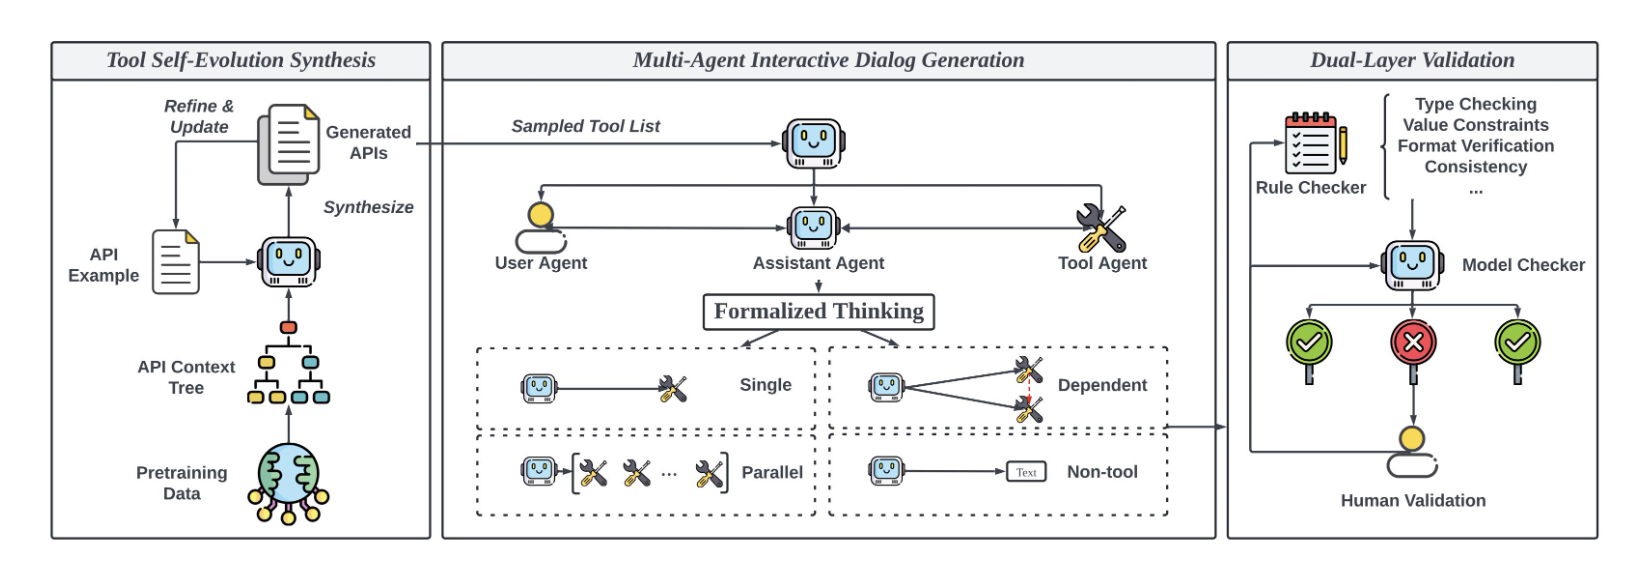
\includegraphics[height=2cm]{../assets/1.png}
%   \hspace{1cm}
%   \includegraphics[height=2cm]{sjtu-vi-badge-red.pdf}
%   \bicaption{中文题图}{English caption}
%   \label{fig:SRR}
% \end{figure}

% 如果多个图形相互独立,并不共用一个图形计数器,那么用 \texttt{minipage} 或者
% \texttt{parbox} 就可以,如图~\ref{fig:parallel1} 与图~\ref{fig:parallel2}。

% \begin{figure}[!htp]
%   \centering
%   \begin{minipage}{0.48\textwidth}
%     \centering
%     \includegraphics[height=1.7cm]{sjtu-vi-name-red.pdf}
%     \caption{并排第一个图}
%     \label{fig:parallel1}
%   \end{minipage}\hfill
%   \begin{minipage}{0.48\textwidth}
%     \centering
%     \includegraphics[height=1.7cm]{sjtu-vi-name-red.pdf}
%     \caption{并排第二个图}
%     \label{fig:parallel2}
%   \end{minipage}
% \end{figure}

% 如果要为共用一个计数器的多个子图添加子图题,建议使用较新的 \pkg{subcaption} 宏
% 包,不建议使用 \pkg{subfigure} 或 \pkg{subfig} 等宏包。

% 推荐使用 \pkg{subcaption} 宏包的 \cs{subcaptionbox} 并排子图,子图题置于子图之
% 下,子图号用 a)、b) 等表示。也可以使用 \pkg{subcaption} 宏包的 \cs{subcaption}
% (放在 minipage中,用法同 \cs{caption})。

% \pkg{subcaption} 宏包也提供了 \pkg{subfigure} 和 \pkg{subtable} 环境,如
% 图~\ref{fig:subfigure}。

% \begin{figure}[!htp]
%   \centering
%   \begin{subfigure}{0.3\textwidth}
%     \centering
%     \includegraphics[height=2cm]{sjtu-vi-badge-red.pdf}
%     \caption{校徽}
%   \end{subfigure}
%   \hspace{1cm}
%   \begin{subfigure}{0.4\textwidth}
%     \centering
%     \includegraphics[height=1.7cm]{sjtu-vi-name-red.pdf}
%     \caption{校名。注意这个图略矮些,subfigure 中同一行的子图在顶端对齐。}
%   \end{subfigure}
%   \caption{包含子图题的范例(使用 subfigure)}
%   \label{fig:subfigure}
% \end{figure}

% 搭配 \pkg{bicaption} 宏包时,可以启用 \cs{subcaptionbox} 和 \cs{subcaption} 的双
% 语变种 \cs{bisubcaptionbox} 和 \cs{bisubcaption},如图~\ref{fig:bisubcaptionbox}
% 所示。

% \begin{figure}[!hbtp]
%   \centering
%   \bisubcaptionbox{$R_3 = 1.5\text{mm}$ 时轴承的压力分布云图}%
%                   {Pressure contour of bearing when $R_3 = 1.5\text{mm}$}%
%                   [6.4cm]{\includegraphics[height=3cm]{example-image-a.pdf}}
%   \hspace{1cm}
%   \bisubcaptionbox{$R_3 = 2.5\text{mm}$ 时轴承的压力分布云图}%
%                   {Pressure contour of bearing when $R_3 = 2.5\text{mm}$}%
%                   [6.4cm]{\includegraphics[height=3cm]{example-image-b.pdf}}
%   \bicaption{包含子图题的范例(使用 subcaptionbox)}
%             {Example with subcaptionbox}
%   \label{fig:bisubcaptionbox}
% \end{figure}


% \section{表格}

% \subsection{基本表格}

% 编排表格应简单明了,表达一致,明晰易懂,表文呼应、内容一致。表题置于表上,研究生
% 学位论文可以用中、英文两种文字居中排写,中文在上,也可以只用中文。

% 表格的编排建议采用国际通行的三线表\footnote{三线表,以其形式简洁、功能分明、阅读
% 方便而在科技论文中被推荐使用。三线表通常只有 3 条线,即顶线、底线和栏目线,没有
% 竖线。}。三线表可以使用 \pkg{booktabs} 提供的 \cs{toprule}、\cs{midrule} 和
% \cs{bottomrule}。它们与 \pkg{longtable} 能很好的配合使用。


% \begin{table}[!hpt]
%   \caption[一个颇为标准的三线表]{一个颇为标准的三线表\footnotemark}
%   \label{tab:firstone}
%   \centering
%   \begin{tabular}{@{}llr@{}} \toprule
%     \multicolumn{2}{c}{Item} \\ \cmidrule(r){1-2}
%     Animal & Description & Price (\$)\\ \midrule
%     Gnat  & per gram  & 13.65 \\
%           & each      & 0.01 \\
%     Gnu   & stuffed   & 92.50 \\
%     Emu   & stuffed   & 33.33 \\
%     Armadillo & frozen & 8.99 \\ \bottomrule
%   \end{tabular}
% \end{table}
% \footnotetext{这个例子来自
%   \href{https://mirrors.sjtug.sjtu.edu.cn/ctan/macros/latex/contrib/booktabs/booktabs.pdf}%
%   {《Publication quality tables in LaTeX》}(\pkg{booktabs} 宏包的文档)。这也是
%   一个在表格中使用脚注的例子,请留意与 \pkg{threeparttable} 实现的效果有何不
%   同。}

% \subsection{复杂表格}

% 我们经常会在表格下方标注数据来源,或者对表格里面的条目进行解释。可以用
% \pkg{threeparttable} 实现带有脚注的表格,如表~\ref{tab:footnote}。

% \begin{table}[!htpb]
%   \bicaption{一个带有脚注的表格的例子}{A Table with footnotes}
%   \label{tab:footnote}
%   \centering
%   \begin{threeparttable}[b]
%      \begin{tabular}{ccd{4}cccc}
%       \toprule
%       \multirow{2}*{total} & \multicolumn{2}{c}{20\tnote{a}} & \multicolumn{2}{c}{40} & \multicolumn{2}{c}{60} \\
%       \cmidrule(lr){2-3}\cmidrule(lr){4-5}\cmidrule(lr){6-7}
%       & www & \multicolumn{1}{c}{k} & www & k & www & k \\ % 使用说明符 d 的列会自动进入数学模式,使用 \multicolumn 对文字表头做特殊处理
%       \midrule
%       & $\underset{(2.12)}{4.22}$ & 120.0140\tnote{b} & 333.15 & 0.0411 & 444.99 & 0.1387 \\
%       & 168.6123 & 10.86 & 255.37 & 0.0353 & 376.14 & 0.1058 \\
%       & 6.761    & 0.007 & 235.37 & 0.0267 & 348.66 & 0.1010 \\
%       \bottomrule
%     \end{tabular}
%     \begin{tablenotes}
%     \item [a] the first note.
%     \item [b] the second note.
%     \end{tablenotes}
%   \end{threeparttable}
% \end{table}


% \section{算法环境}

% 算法环境可以使用 \pkg{algorithms} 宏包或者较新的 \pkg{algorithm2e} 实现。
% 算法~\ref{algo:algorithm} 是一个使用 \pkg{algorithm2e} 的例子。关于排版算法环境
% 的具体方法,请阅读相关宏包的官方文档。

% \begin{algorithm}[htb]
%   \caption{算法示例}
%   \label{algo:algorithm}
%   \small
%   \SetAlgoLined
%   \KwData{this text}
%   \KwResult{how to write algorithm with \LaTeXe }

%   initialization\;
%   \While{not at end of this document}{
%     read current\;
%     \eIf{understand}{
%       go to next section\;
%       current section becomes this one\;
%     }{
%       go back to the beginning of current section\;
%     }
%   }
% \end{algorithm}


\section{本章小结}


\chapter{知识图谱与大语言模型互增益的API编排方法}

\section{引言}
\label{sec:intro}

\subsection{问题构建}

工具增强的 LLM 通过结构化的自然语言文本与环境进行交互。一般的交互过程可以描述如下:在步骤 \( s \) 时,LLM 接收当前环境观察 \( o_s \) 以及交互活动历史 \( C_s \) 作为输入,并产生一个语言思维 \( t_s \in L \)。然后,LLM 通过采取一个动作 \( a_s \in A \) 与环境进行交互,该动作可以描述为一个工具名称及其参数的元组,例如 \( a_s = (tools, args) \),其中 \( tools \in T \)。随后,LLM 从环境 \( E \) 中获取新的观察 \( o_{s+1} \)。通过迭代这个交互过程,LLM 最终可能解决给定的任务。

LLM 大多是无状态的。交互历史 \( C_s \) 通常作为 LLM 输入的一部分,帮助 LLM 回忆之前的过程并推断下一个动作 \( a_{s+1} \)。我们将 \( C_s \) 定义为大小为 \( K \) 的队列,包含过去的观察、思维和动作,例如 

\[
C_s = [(o_{s-k}, t_{s-k}, a_{s-k}), \ldots, (o_{s-1}, t_{s-1}, a_{s-1})].
\]

在每一步中,新的思维、动作和观察的元组被附加到 \( C_s \) 中;如果达到最大容量,最早的元组将被弹出。

除了 \( C_s \),可用工具集合 \( T \) 也需要作为输入上下文的一部分,其中 LLM 可以选择一个合适的工具。设 \( P_\theta \) 表示具有参数 \( \theta \) 的工具增强 LLM。严格地说,上述交互过程可以形式化为以下公式:

\[
t_s = P_\theta(C_s \cup o_s) \tag{1}
\]

\[
a_s = P_\theta(C_s \cup o_s, t_s, T) \tag{2}
\]

\[
o_{s+1} = E(a_s) \tag{3}
\]

现有工具增强 LLM 的一个主要问题是它们的重 token 消耗,这在很大程度上归因于 \( C_s \) 和 \( T \) 的长输入上下文。一种代表性的解决方案是将 \( C_s \) 的长文本分段并压缩为语义嵌入。随后,可以计算并排名候选段落与当前观察 \( o_s \) 之间的语义相似度分数。最后,公式 (1) 和 (2) 中的 \( C_s \) 被替换为与 LLM 输入最相关的段落。直观上,这一解决方案可以扩展到 \( T \),例如,搜索与思维 \( t_s \) 最相关的工具。然而,根据公式 (1),\( t_s \) 的生成并不具备关于 \( T \) 的全面知识。\( t_s \) 中的语义信息可能与 \( T \) 中的任何工具无关。此外,在大量 API 函数的库中,可能有许多工具共享类似的语义信息,但功能上略有不同。当 \( |T| \) 变大时,通过语义嵌入搜索工具可能会粗糙且不准确。因此,现有的工具学习方法要么局限于数量有限的专门设计的工具,要么使用指令微调来增强 LLM \( P_\theta \) 以包含 \( T \) 的先验知识,这在计算上可能是资源密集型的。

\subsection{基于深度优先遍历的动态搜索算法}

为了更好地利用我们构建的工具图谱,并挖掘隐藏节点关系中的知识,我们开发了一个基于深度优先遍历的寻路算法。与“思维链”(Chain-of-Thought)或ReACT方法相比,该算法的优点在于能够防止错误传播,并对整体工具行动空间进行更深入的探索。

我们提出的基于深度优先的寻路算法的流程图如下所示:

首先,由于图谱上的节点数量众多,选择初始节点是算法中非常关键的一步。在选择初始节点时,我们利用基于语义相似度的API召回器,得到与用户需求在语义上最相似的一组工具,让大语言模型进行选择,最终确定初始节点,并从该节点开始进行后续探索。

其次,我们在图上构建一棵深度优先搜索树,允许模型在图上不断选择新的节点并评估每一条推理路径。具体逻辑如下:对于每个选择的节点,我们调用该节点并获取对应的API响应内容,然后将已经调用的工具轨迹、解析后的API响应、用户需求等提供给大语言模型,让模型选择下一步操作。下一步操作可以是继续选择节点,也可以是回溯到上一节点。

如果模型选择了下一步操作,我们将获取当前节点的邻居节点及其权值,并提供给大模型智能体。对于邻居节点的选择,我们会获取到当前节点权值最大的5个节点作为下一步操作。如果邻居节点不足5个,我们将重新调用API召回器,以补全5个选择的选项。模型会根据当前状态继续迭代选择,直到结束选择或放弃。

如果模型选择回溯到上一节点,我们将在短期记忆模块中添加回溯步骤,并恢复到上一个节点的状态。将回溯步骤添加到短期记忆的原因是让模型记住在本次推理中之前采取的错误操作,避免后续重复选择不可行的工具。如果模型回溯到了初始节点,并且需要继续回溯,我们可以理解为基于当前的工具组,该任务不可行,即放弃任务执行。

\begin{algorithm}[htb]
    \caption{图谱节点选择算法}
    \label{algo:algorithm}
    \small
    \SetAlgoLined
    \KwData{用户需求 $user需求$}
    \KwResult{选择合适的工具}
  
    // 选择初始节点\;
    $initialNodes \gets API召回器(user需求)$\;
    $selectedNode \gets LLM选择初始节点(initialNodes)$\;
    
    // 初始化深度优先搜索树\;
    $dfsTree \gets \text{new Tree()}$\;
    $dfsTree.addNode(selectedNode)$\;
  
    \While{true}{
      $response \gets 调用API(selectedNode)$\;
      
      // 提供信息给大语言模型\;
      $状态信息 \gets \{\text{工具轨迹}, \text{API响应}, \text{用户需求}\}$\;
      $nextAction \gets LLM选择下一步操作(状态信息)$\;
  
      \eIf{nextAction == "选择下一节点"}{
        $topNeighbors \gets 选择邻居节点(selectedNode)$\;
        \If{length(topNeighbors) < 5}{
          $topNeighbors \gets API召回器补全选择(selectedNode)$\;
        }
        $selectedNode \gets LLM选择下一个节点(topNeighbors)$\;
        $dfsTree.addNode(selectedNode)$\;
      }{
        // 回溯逻辑\;
        $短期记忆.add回溯步骤(dfsTree.currentNode())$\;
        $selectedNode \gets dfsTree.backtrack()$\;
  
        \If{selectedNode == dfsTree.root() \&\& 需要继续回溯()}{
          放弃任务()\;
          break\;
        }
      }
      
      \If{模型结束选择()}{
        break\;
      }
    }
  \end{algorithm}

\subsection{基于反思机制的回溯算法}

\subsection{工具调用路径长短期记忆框架}

\subsubsection{长短期记忆框架概述}

本小节提出了关于增强模型规划和推理准确性的长短期记忆框架。该框架主要分为短期记忆和长期记忆两个部分。短期记忆部分指的是当模型在图上动态推理时存储的每个步骤的记录,主要聚焦于以什么数据格式来存储推理步骤,以及记录哪些有用的记忆信息:在图上前进、回溯还有大模型的思考过程等。长期记忆部分主要有记忆存储、召回和利用三个部分,围绕着如何进一步利用过去成功推理的经验来辅助后续的推理和规划过程。

\subsubsection{短期记忆}

短期记忆指的是模型在图上进行不断推理时保存的一些状态信息,这些信息包括:用户的任务、当前遍历到的节点、历史遍历的节点、轨迹路径信息等。在遍历的过程中,我们会动态地更新和维护短期记忆存储的内容,来辅助模型进行推理和规划。在短期记忆中,我们一般将全部的信息存储在内存中,然后直接构建提示词添加到大语言模型的上下文中,让模型能够感知到当前的状态和环境。

\subsubsection{长期记忆}

长期记忆是与短期记忆相对的概念,长期记忆会固定地存在数据库中,并且随着调用次数增多而积累。长期记忆记录的是最终形成的工具调用链以及结果,每次在系统进行推理时都会从长期记忆库中进行搜索,从而利用历史经验知识来辅助模型的推理。

长期记忆的具体实现方式如下,包括记忆的添加、删除、修改和查询四个部分。

\begin{enumerate}
    \item \textbf{记忆添加} \\
    记忆增加是该框架中最基础的功能。首先,除了初始记忆批量添加的阶段,其他的记忆添加都是在生成了新的推理路径时进行。我们先对新生成的推理路径进行筛选,通过一个评判器来对推理路径判断质量。如果评判器认定为“失败”或“不确定”,那么就舍弃当前的推理路径。这一步的判别是为了保证记忆的质量,不存储有失败风险的路径在记忆中。随后,我们将用户的需求与推理路径形成一个二元组,将用户需求输入向量模型转为嵌入向量,将推理路径作为文本格式存储,方便计算和检索记忆。

    \item \textbf{记忆修改} \\
    对于同一个任务,系统可能会生成不同的推理路径。在这种情况下,我们会用新的记忆来替换旧的记忆,对记忆做出及时的更新。在记忆修改时,我们只需要对推理路径部分进行修改,并保存更新后的路径在数据库中,而不需要对用户需求的向量部分进行修改。

    \item \textbf{记忆删除} \\
    由于工具节点的状态是随时变化的,比如开发者停止维护了某个工具,或者是某个工具 API 出现故障等等,因此有的时候我们会删除一些工具节点或修改节点状态为“失效”。在这种情况下,我们除了在工具图谱上进行修改,也应该同时删除有关的记忆,避免对模型造成困扰。记忆删除的逻辑较为清晰,即当某工具被删除或失效时,在记忆库中匹配所有包含该工具的路径并删除对应的记忆。

    \item \textbf{记忆查询} \\
    在有新的用户需求时,系统会首先将用户需求转为向量形式,然后在向量数据库中通过相似度检索算法查找到与当前需求最相似的 K 个历史需求以及对应的工具轨迹,即搜索得到的记忆。
\end{enumerate}

\subsubsection{记忆搜索与召回}
\subsubsection{记忆利用}
(可以做消融实验)

\section{真实工具调用模拟}
\label{sec:real_tool_simulation}

\section{实验与评估}
\subsection{测试数据集}
\label{subsec:test_dataset}

ToolBench。ToolBench\cite{Qin2023}是一个公开的针对工具调用的数据集,其中包含了来自49个类别的16464个真实世界的API工具的推理轨迹数据。该数据集包括三个部分,三个子数据集的难度逐级上升:G1数据集,其中目标任务所需的API都在同一个工具组;G2数据集,其中目标任务所需的API在同一个类别但是属于不同的工具组;G3数据集,其中目标任务所需的API会跨越不同类别。为了测试各个难度等级上的能力,本工作从三个类别分别抽取了350,350和300条数据构建测试集。测试集一共涉及18个category的358个工具。

API-Bank。API-Bank\cite{Li2023}是另一个公开的工具调用数据集,作者们针对模型工具调用的检索、规划能力的评估精心构建了测试数据,其中包含73个API工具,并对314个工具调用进行了标注。本工作从中抽取了300条数据作为测试集。

\subsection{评估指标}
由于工具的多样性,对于同一个用户需求可以有多种工具调用路径。因此,我们无法事先对每个测试的输入标注单一的解决路径标准答案。由于人工评价较为费时费力,本文基于\cite{Tang2023}中的评估器构建了类似的评估体系,包含以下两个指标。我们的评估器使用的是目前能力最强的模型之一GPT-4,温度系数设置为0。(todo)

\begin{itemize}
    \item \textbf{通过率(Pass Rate)} \\
    通过率是计算在有限的工具执行步骤内完成了需求的比例。该指标衡量了系统工具调用最基本的执行能力。通过率的公式如下:

    \begin{equation}
        PR = \frac{ \#(\text{Solved}) }{ \#(\text{Solved}) + \#(\text{Unsolved}) }.
    \end{equation}

    \item \textbf{胜率(Win Rate)} \\
    胜率是评价两条针对同一需求生成的路径的偏好。在模型判断胜率的评估器的提示词中,我们预先定义了一组标准,其中包括:探索性、真实性、工具个数。胜率的公式如下:

    \begin{equation}
        WR = \frac{ \#(\text{Won}) }{ \#(\text{Won}) + \#(\text{Lost}) + \#(\text{Tie}) }.
    \end{equation}

\end{itemize}

同时,为了验证评估器与人类标注者的标注一致性,我们人工标注了100条通过率和100条胜率的数据。经过这200条数据,我们发现标注器在通过率上与人工标注的一致性达到了xxx(todo),在胜率上该数字达到了xxx(todo),这表明该基于大语言模型的标注器与人工标注的标准基本吻合。

\subsection{实验结果}
我们在不同基模型上测试了不同的工具编排调用方式并与我们的方法进行对比。
\begin{itemize}
    \item 基准线:其他的vanilla、cot、react的prompt等。
\end{itemize}

\subsection{实验分析}
\label{subsec:exp_analysis}

\section{本章小结}
\label{sec:summary_chap4}
% !TeX root = ../main.tex

\chapter{系统设计与实现}

本章设计并实现了一个具有交互性和用户友好性的基于知识图谱和大语言模型智能体机制的API编排和调用系统。该系统集成了不同模型的调用接口,以及知识图谱查询的功能。该系统提供了一个使用门槛低、用户友好的界面,允许用户通过自然语言的方式与该系统进行交互和提问,系统会根据用户的需求编排并调用所需的API,并进行回答。

难点:

界面设计:友好交互、展示图谱部分、添加api部分

前后端框架选什么

前:streamlit 后:fastapi


模型管理(不同模型,超参数,上下线) 如何交互 容错 restapi格式 如何加速

数据管理 neo4j qdrant 用户数据 记忆数据

\section{系统需求分析}

\indent 我们采用面向对象的需求分析方法,绘制了如图所示的系统用例图。

“如图~\ref{fig:usecase} 所示”等。该页空
白不够排写该图整体时,则可将其后文字部分提前排写,将图移到次页。

\begin{figure}[!htp]
  \vspace{1em}
  \centering
  \setlength{\abovecaptionskip}{10pt} % 控制图片和caption之间的距离
  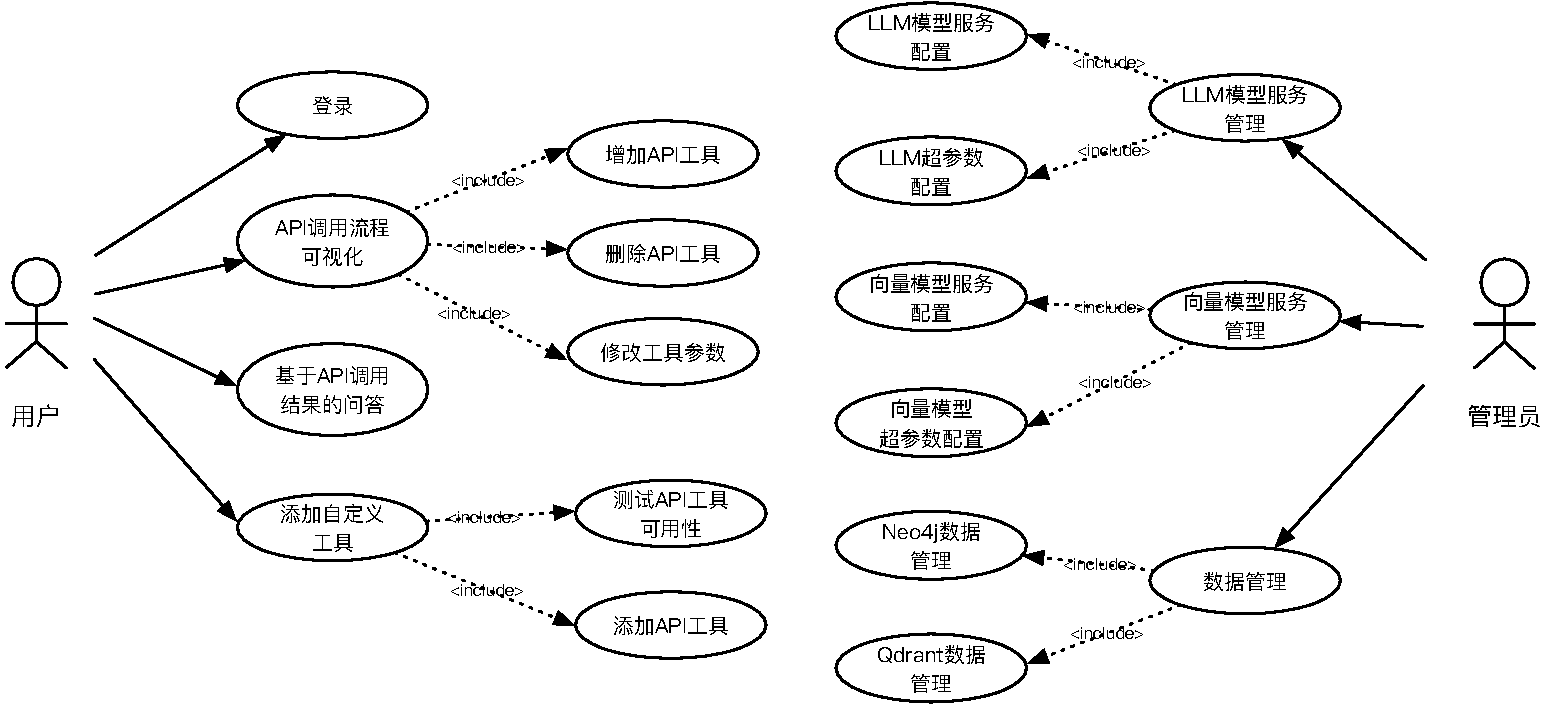
\includegraphics[height=7cm]{../assets/ch5-用例图.pdf}
  \bicaption{系统用例图}{System Usecase Diagram}
  \label{fig:usecase}
\end{figure}

在用例图中,我们定义了两种角色:系统用户和管理人员。从需求出发,系统应该实现以下功能:

针对普通用户的功能:

1. 登录功能

2. API调用流程可视化

3. 基于API调用结果的问答

4. 添加自定义工具

针对管理员的功能:

1. 大语言模型服务管理

2. 向量模型服务管理

3. 数据管理

在该系统中,基于大语言模型的智能体可以通过多轮对话的交互方式与用户进行交流,并通过解析用户的需求来提供对应的工具调用流程和根据工具调用结果得到的总结回复

本文的系统提供的主要功能是根据用户需求得到调用流程并执行,从而给用户提供有效的信息。针对该核心功能,我们针对不同用户群体设计了两种使用的模式:对于有计算机编程基础的用户,我们提供了开发者模式,即用户可以自己对工具执行流程进行编辑和调整,以确保更加符合其查询需求;对于一般用户,我们按照系统生成的流程进行执行,得到最终结果。除了该功能外,本系统还提供了自定义工具添加、工具模板库浏览等功能。

\section{系统设计与架构}
本文设计的基于知识图谱和智能体的API编排与调用系统,整体的系统框架设计如图xx所示。系统主要包含四层:数据管理层、API编排层、API调用层和UI层。

\subsection{交互方案设计}


\subsection{系统架构设计}

\indent 本系统的架构将会从部署架构和软件架构来进行说明。

部署架构。

软件架构。


\subsection{数据管理层}
数据管理层主要负责下列内容的存储:
\begin{enumerate}
    \item API知识图谱的存储
    \item 向量形式存储的API详细信息,这些预先计算并存储在向量数据库中,便于快速计算
    \item 系统使用过程中的历史推理轨迹的存储,作为经验数据供后续参考
\end{enumerate}

\subsection{API编排层}
API编排层主要实现本系统的动态API编排功能。该层主要包括以下几个部分:
\begin{enumerate}
    \item \textbf{用户需求拆解模块}:通过大语言模型智能体机制,将用户的复杂、完整需求拆解为多个子需求,并对子需求逐一调用。
    \item \textbf{API推理轨迹检索模块}:根据子任务的任务描述,检索历史推理轨迹中相似任务,提供参考。
    \item \textbf{API知识图谱检索模块}:根据不同的检索模式,搜索API节点及相关信息作为返回。
    \item \textbf{基于图谱的DFS动态编排算法模块}:在知识图谱上进行搜索和回溯,得到最终的调用路径。
\end{enumerate}
该层的主要流程为:首先通过拆解模块将任务拆解为独立的子任务,然后针对每个子任务,检索类似任务作为参考,并检索相关API信息,构建提示词,基于大模型的推理能力和上下文生成结构化的API流程。

\subsection{API调用层}
API调用层主要负责根据API编排层生成的调用流程,获取调用参数并执行API调用。主要涉及到以下部分:
\begin{itemize}
    \item \textbf{API参数获取模块}: 首先,我们获取得到对应API的参数信息以及用户的具体需求,提供给大语言模型让模型给出API所需的输入参数。
    \item \textbf{API调用模块}: 在该部分,会使用API参数获取模块的参数作为API输入来调用工具API,若执行成功则将JSON格式的调用结果传递到API调用结果总结模块。该部分设置了自动重试机制,若调用失败则自动重试3次,如果3次都失败则返回错误信息。
    \item \textbf{API调用结果总结模块}: 在执行并得到了API的调用结果后,将所有的API执行结果转化为自然语言的格式,将这些执行结果和用户原需求输入基于大语言模型的总结模块获取最终自然语言格式的总结内容。
\end{itemize}

\subsection{UI层}
UI层是web前端页面,负责与用户直接交互,提供用户友好的界面。不同页面对应不同功能:
\begin{itemize}
    \item \textbf{信息问答页面}:用户通过自然语言输入具体的需求,然后系统会进行API调用路径的编排并依次调用,最终将总结好的自然语言文本的结果也提供给用户。整体的交互方式与大模型多轮对话是相似的。
    \item \textbf{自定义API添加页面}:用户可以通过填写API的详细信息,如API的名称、API的调用链接、API的具体参数类型和参数描述信息等添加新的API。添加新API后还需要经过测试,确保API调用的有效性再添加到API仓库中。
    \item \textbf{API历史调用参考页面}:用户可以可视化的形式浏览历史API调用记录,并通过选择和配置参数的方式再次调用历史API调用链。
\end{itemize}
UI层代码是基于streamlit代码库实现的。

\subsection{模块设计}

图xx展示了系统详细的功能层次结构。本系统的详细功能主要包含:用户验证、数据管理、模型服务管理、API工作流编排、API调用问答、自定义API存储。

\subsection{用户验证}
用户验证模块用于实现面向用户的API调用历史记录和模板库构建。该模块包含用户注册和登录功能,允许用户通过注册获得个人账号并登录系统使用。

\subsection{数据管理}
数据管理模块用于管理系统中的各类数据,包括知识图谱数据、API信息向量以及用户交互过程中的历史需求、API编排和调用结果等。主要存储在neo4j和Qdrant向量数据库中。

\subsection{模型服务管理}
模型服务管理模块包括模型接口封装和模型超参数配置功能。封装不同模型的调用代码为统一接口,对系统其他部分隐藏模型的具体细节。超参数配置则管理模型调用时的参数,如温度系数、最大长度、top\_k、top\_p等。

\subsection{API工作流编排}
API工作流编排模块包含以下三个子模块:
\begin{itemize}
    \item \textbf{编排模式选择}:提供用户可配置的编排选项。
    \item \textbf{编排结果展示}:通过可编辑任务框展示API编排结果,任务框中展示API名称、描述、参数等信息。
    \item \textbf{API流程自定义}:允许用户在生成的API流程基础上,进行增加、删除或修改,支持更灵活的API调用。
\end{itemize}

\subsection{API调用问答}
API调用问答模块通过流式输出和多轮交互,提升用户体验。流式输出模块增强用户等待结果时的体验,多轮交互模块保存上下文中的API调用结果,支持进一步提问。

\subsection{自定义API存储}
自定义API存储模块通过API添加和测试模块,支持用户将自定义API添加到系统中,提高系统扩展性和可用性。

\section{系统实现}

技术选型。

\section{系统展示}
(此处为系统截图展示)

\section{本章小结}
\chapter{系统设计与实现}

本章设计并实现了一个具有交互性和用户友好性的基于知识图谱和大语言模型智能体机制的API编排和调用系统。该系统集成了不同模型的调用接口,以及知识图谱查询的功能。该系统提供了一个使用门槛低、用户友好的界面,允许用户通过自然语言的方式与该系统进行交互和提问,系统会根据用户的需求编排并调用所需的API,并进行回答。

难点:

界面设计:友好交互、展示图谱部分、添加api部分

前后端框架选什么

前:streamlit 后:fastapi


模型管理(不同模型,超参数,上下线) 如何交互 容错 restapi格式 如何加速

数据管理 Neo4j qdrant 用户数据 记忆数据

\section{系统需求分析}

\indent 我们采用面向对象的需求分析方法,绘制了如图~\ref{fig:usecase}所示的系统用例图。

\begin{figure}[!htp]
  \vspace{1em}
  \centering
  \setlength{\abovecaptionskip}{10pt} % 控制图片和caption之间的距离
  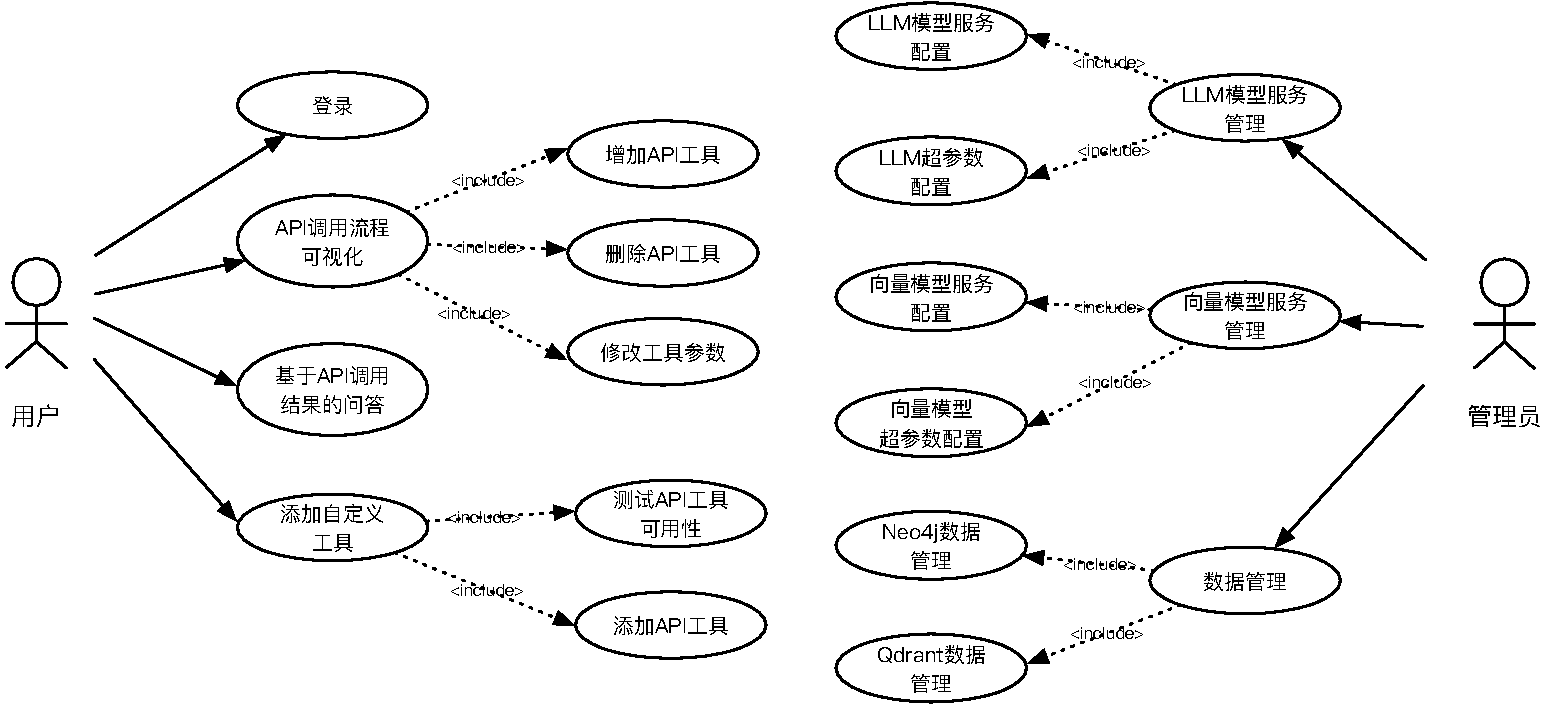
\includegraphics[height=6cm]{../assets/ch5-用例图.pdf}
  \bicaption{系统用例图}{System Usecase Diagram}
  \label{fig:usecase}
\end{figure}

我们采用面向对象的需求分析方法,绘制了系统的用例图。在该用例图中,我们定义了两种主要角色:系统用户和管理人员。系统用户包含普通用户和开发者,而管理人员则具有更高权限的管理功能。这样的角色划分帮助系统满足不同用户的需求,支持工具调用、数据管理、模型管理等任务。根据需求分析,系统应具备以下核心功能模块:

1.	用户与权限管理:系统应提供用户注册、登录、身份验证和权限分配功能。系统用户可根据权限访问相应模块,而管理人员具有配置用户权限的能力,以保障系统安全性和合理性。

2.	API调用流程管理与问答支持:系统支持用户通过可视化界面查看并编辑API调用流程,并能基于调用结果进行问答。API调用流程管理模块可展示调用步骤、输入输出等信息,用户可根据需要进行简单调整。问答模块则负责对编排好的工具流程进行调用和解析,生成总结性描述或回答用户问题。

3.	自定义工具与工具库管理:系统支持用户根据需求添加自定义工具,丰富工具库的扩展性。用户通过填写工具的配置信息并测试后,系统将自动集成到工具库,供用户选择和调用。同时,工具库还提供常用工具模板,方便用户浏览和直接调用。

4.	模型服务管理:系统为管理人员提供大语言模型和向量模型服务的管理功能。该模块支持模型的配置、更新和监控,以满足多种任务需求并优化系统性能。管理人员可以根据需要对模型进行更新,以确保系统提供高效的模型服务。

5. 数据库管理:系统应提供高效的图数据库和向量数据库管理功能,以支持管理员对不同类型的数据进行配置和管理。对于图数据库管理,平台应支持Neo4j等图数据库的配置,允许管理员查看数据库状态、管理数据结构和优化查询性能,以确保关系数据的高效存储和检索。对于向量数据库管理,平台应支持Qdrant等向量数据库的配置,允许管理员调整存储策略和搜索参数,以优化向量数据的存储和检索性能。系统支持大规模向量数据的导入、分片配置和索引更新,确保能够高效完成相似度计算,满足推荐系统和语义搜索等场景的需求。

\section{交互方案设计}

图~\ref{fig:system}为该系统的交互设计图。

\begin{figure}[!htp]
    \vspace{1em}
    \centering
    \setlength{\abovecaptionskip}{10pt} % 控制图片和caption之间的距离
    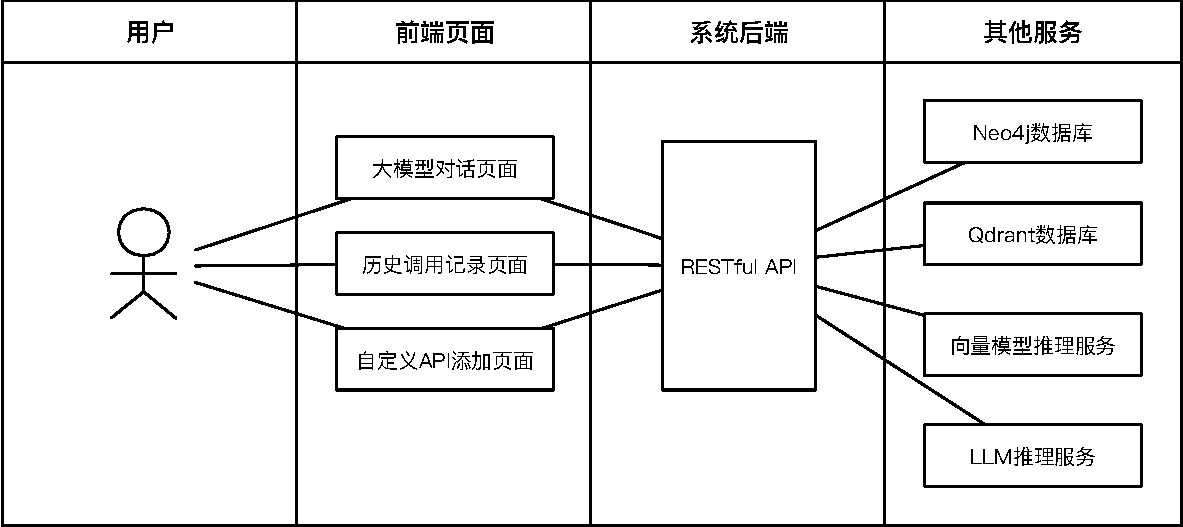
\includegraphics[height=5cm]{../assets/ch5-交互设计图.pdf}
    \bicaption{系统交互图}{System Usecase Diagram}
    \label{fig:interaction}
  \end{figure}


本系统主要有以下三个部分,前端交互界面、系统后端和其他服务模块,集成了不同模型的调用接口以及知识图谱查询功能,为用户提供了低门槛、用户友好的界面,支持用户通过自然语言的方式进行交互和提问。整体交互流程如图6.2所示:

	1.	前端页面:前端页面为用户提供了交互界面,支持大模型对话、历史调用记录以及自定义API工具添加等功能。用户可以通过这些页面与系统进行自然语言交互,例如通过对话界面向大模型提问、查看历史调用模板获取API使用信息,或在自定义页面添加新的API工具以扩展系统功能。
	2.	系统后端:系统后端作为核心控制层,通过RESTful API接口将前端用户请求传递至其他服务模块,并负责业务逻辑的处理。后端系统不仅管理用户请求的权限和数据存储,还充当API编排的核心,确保前端请求的安全性和规范性。在与其他服务模块的交互中,后端可以灵活调用图数据库、向量数据库以及模型推理服务,实现对知识图谱的查询和不同模型的协同调用,以满足复杂的查询和推理需求。
	3.	其他服务模块:其他服务模块包括Neo4j图数据库、Qdrant向量数据库、向量模型推理服务和LLM(大语言模型)推理服务。这些模块分别用于存储和查询图数据库、管理和检索向量化数据、支持基于向量相似度的搜索需求,以及提供大语言模型的对话和推理功能。系统后端根据用户需求对这些服务进行编排调用,确保用户问题得到高效而准确的解答。

通过以上三部分的协同工作,系统能够为用户提供全面的API编排调用智能问答、历史调用模板查询和自定义工具配置等服务,满足用户的需求,并提供了易用、易扩展的系统和良好的交互体验。


\section{系统架构设计}

本系统架构分为五个层次:存储层、访问层、功能层、接口层和展示层。以下对各层的功能和组成模块进行详细介绍。

图~\ref{fig:system}为该系统的系统软件架构设计图。

\begin{figure}[!htp]
    \vspace{1em}
    \centering
    \setlength{\abovecaptionskip}{10pt} % 控制图片和caption之间的距离
    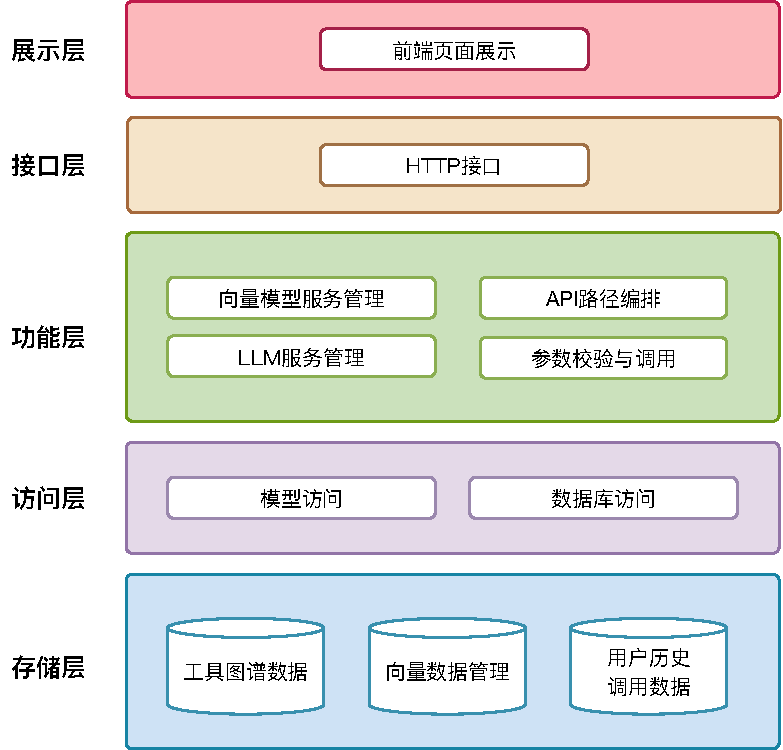
\includegraphics[height=8cm]{../assets/ch5-系统架构图.pdf}
    \bicaption{系统用例图}{System Usecase Diagram}
    \label{fig:system}
  \end{figure}

\subsection{存储层}

存储层负责系统核心数据的存储,包括以下内容:
\begin{itemize}
    \item \textbf{API知识图谱}:用于存储API的知识关联信息,方便后续的关系检索和动态编排。
    \item \textbf{API详细信息的向量存储}:将API的详细信息预先计算并存储在向量数据库中,以便于快速计算相似度。
    \item \textbf{历史调用路径}:记录系统使用过程中产生的调用路径,作为经验数据供后续参考和优化。
\end{itemize}

\subsection{访问层}

访问层负责封装对存储层的访问功能,提供统一的数据访问接口,便于功能层的调用。其主要功能包括:
\begin{itemize}
    \item 访问图数据库和向量数据库的数据,进行知识图谱检索和相似性计算。
    \item 访问和解析JSON格式的文件数据,确保数据在各层之间的顺畅传递。
\end{itemize}

\subsection{功能层}

功能层是系统的核心,实现动态API编排和调用。主要模块包括:

\begin{itemize}
  \item \textbf{任务分解模块}:输入用户的复杂需求,输出为拆解后的固定格式的一组子任务,子任务之间相互独立。
  \item \textbf{长期记忆检索模块}:根据当前任务描述,在历史调用路径中检索相似任务描述和历史调用路径,提供给当前任务的动态API编排模块作为参考。
  \item \textbf{API知识图谱检索模块}:按照不同的检索模式搜索API节点及其关联的邻居节点信息。
  \item \textbf{基于图谱的DFS动态编排算法模块}:在知识图谱上执行深度优先搜索和回溯操作,生成最优的调用路径。
  \item \textbf{API调用模块}:获取目标API的参数信息,并结合用户需求生成API调用的输入参数。使用生成的参数调用API,同时设置自动重试机制,以确保调用的稳定性;若调用失败则进行重试,若多次重试仍失败则返回错误信息。
  \item \textbf{API调用结果总结模块}:将API调用结果转换为自然语言格式,并结合用户的原始需求生成最终的总结性回复。
\end{itemize}

\subsection{接口层}

接口层负责为系统各功能提供访问接口,采用RESTful API的HTTP接口形式:
\begin{itemize}
    \item 系统后端通过RESTful API接口与前端交互,供前端进行数据访问和操作。
    \item 模型服务与平台后端之间也通过HTTP接口进行通信,以确保数据传输的安全性和高效性。
\end{itemize}

\subsection{展示层}

展示层是面向用户的web前端页面,为用户提供直观友好的交互界面。主要页面包括:
\begin{itemize}
    \item \textbf{信息问答页面}:用户可通过自然语言输入需求,系统将自动编排API调用路径并执行,最终以自然语言格式返回结果,模拟多轮对话的交互体验。
    \item \textbf{自定义API添加页面}:用户填写API名称、调用链接、参数类型和描述信息等来添加新API。新API需经过测试验证后方可加入API仓库。
    \item \textbf{API历史调用参考页面}:用户可以查看历史API调用记录,并支持通过选择和配置参数重新使用历史API调用链。
\end{itemize}

\section{模块设计}

图~\ref{fig:module}展示了系统详细的功能层次结构。本系统的详细功能主要包含:用户验证、数据管理、模型服务管理、API工作流编排、API调用问答、自定义API存储。

\begin{figure}[!htp]
  \vspace{1em}
  \centering
  \setlength{\abovecaptionskip}{10pt} % 控制图片和caption之间的距离
  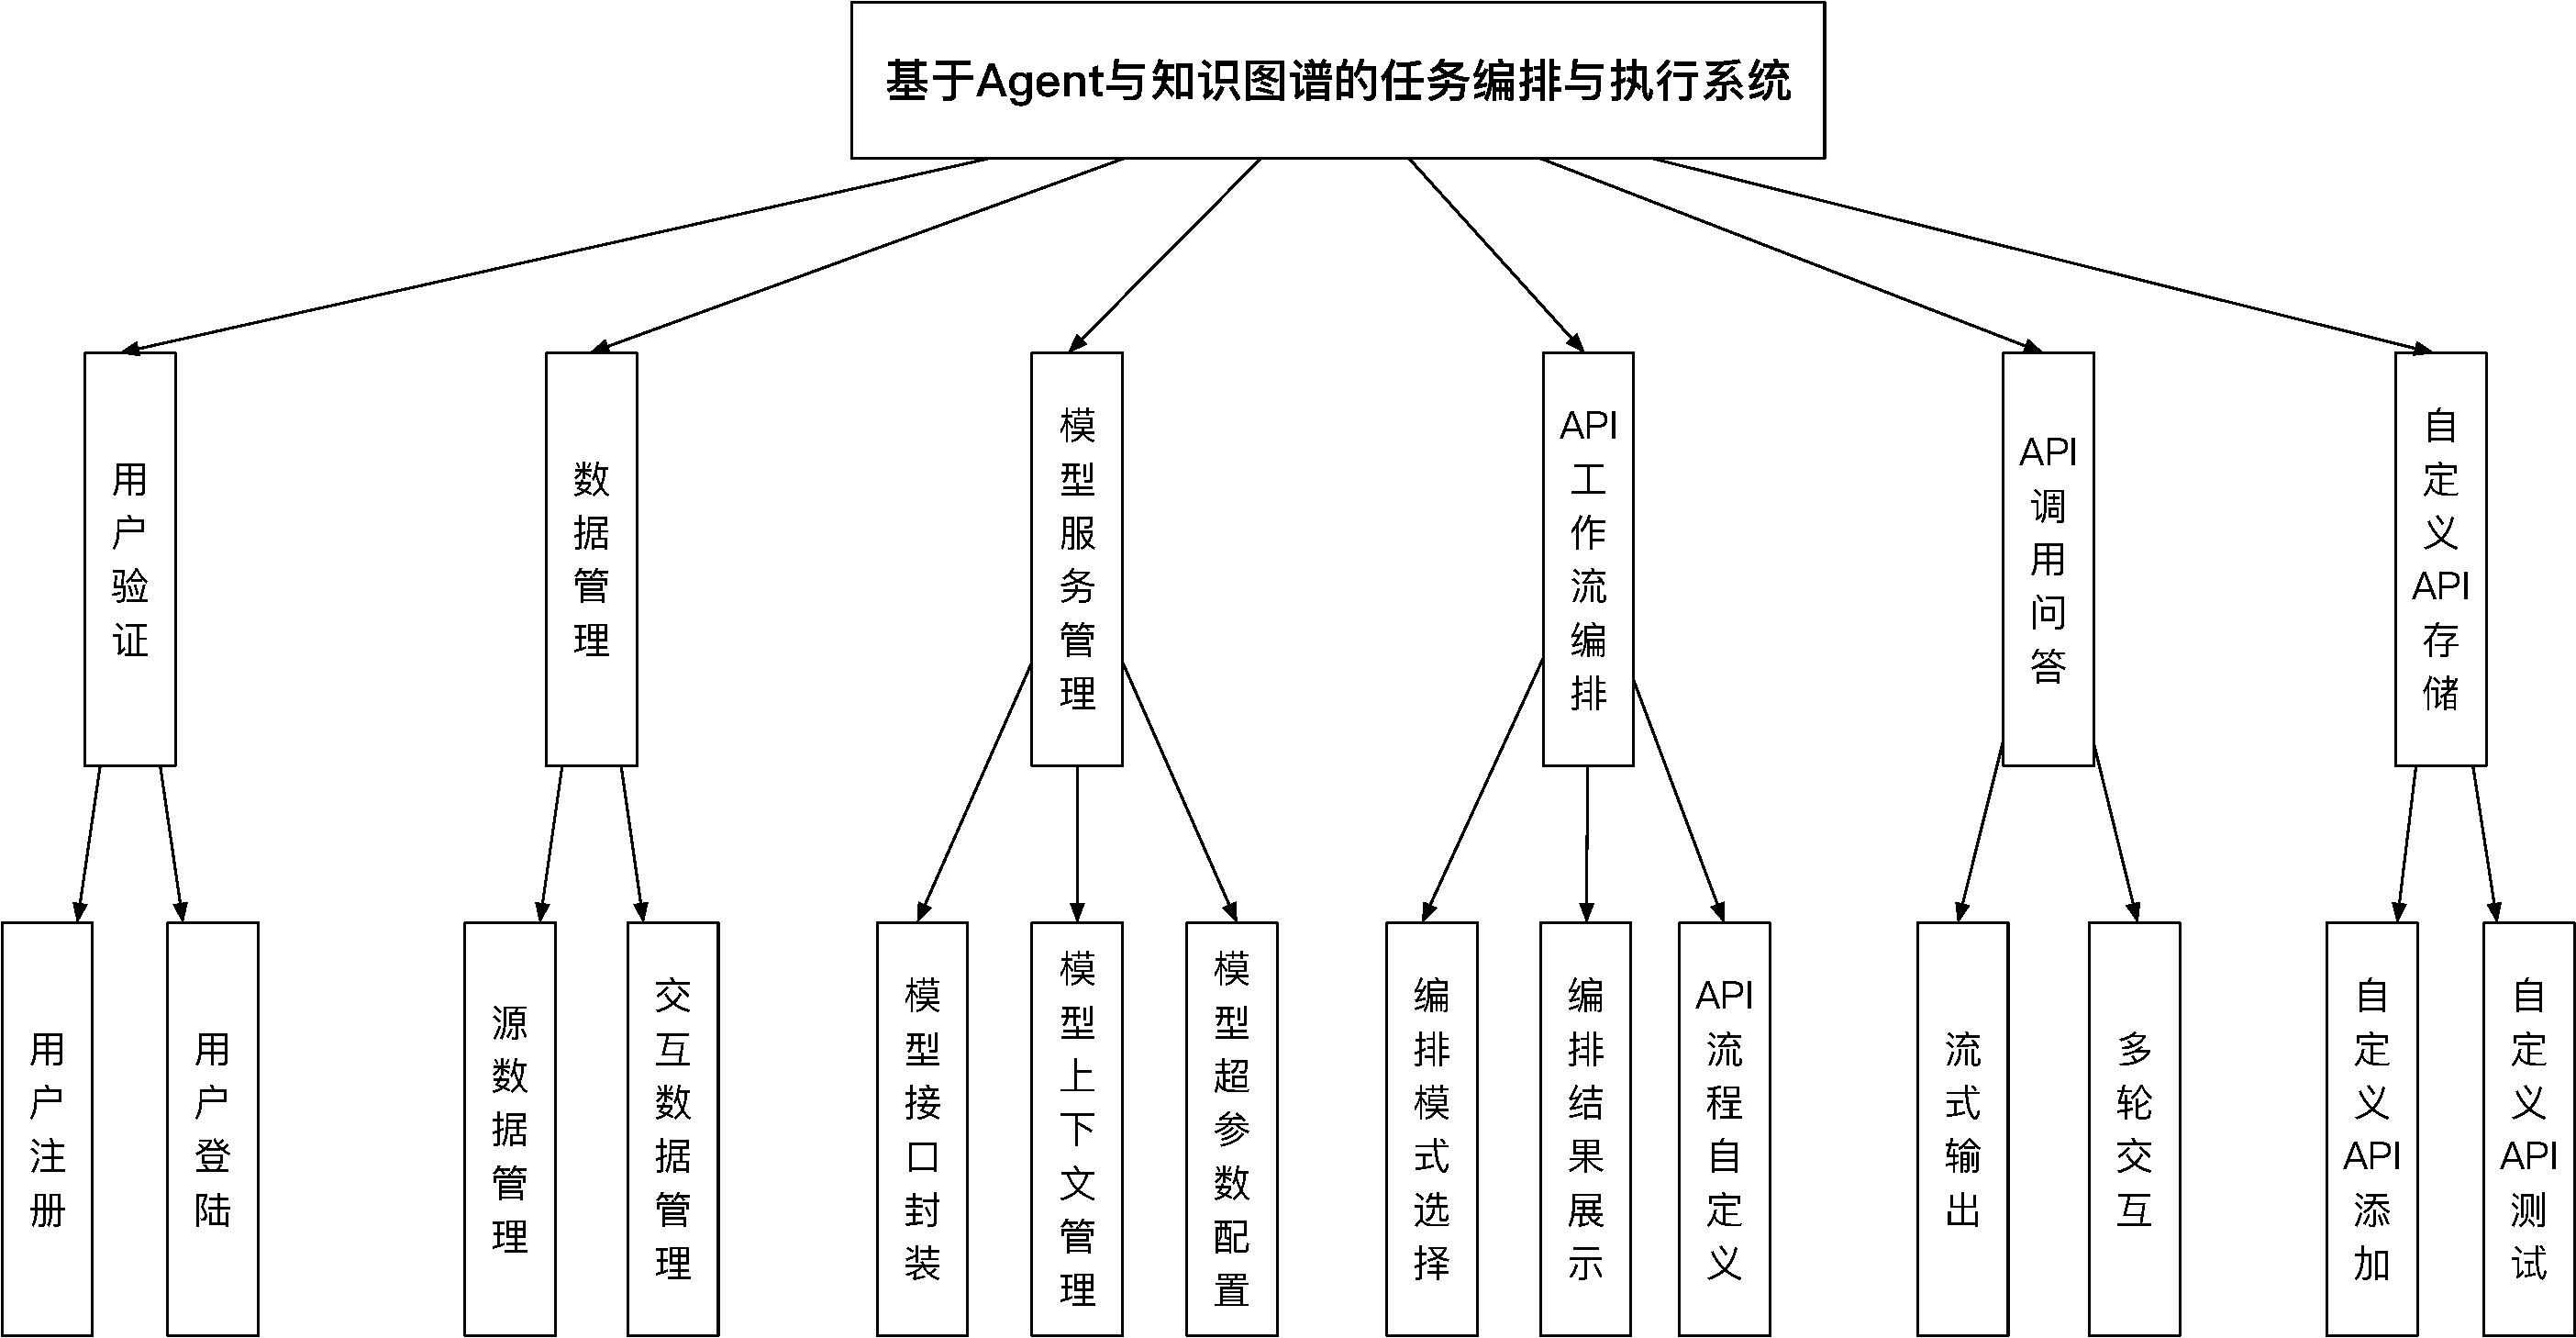
\includegraphics[height=7cm]{../assets/ch5-系统模块图.pdf}
  \bicaption{系统模块图}{System Module Diagram}
  \label{fig:module}
\end{figure}

\subsection{用户验证}
用户验证模块用于实现面向用户的API调用历史记录和模板库构建。该模块包含用户注册和登录功能,允许用户通过注册获得个人账号并登录系统使用。

\subsection{数据管理}
数据管理模块用于管理系统中的各类数据,包括知识图谱数据、API信息向量以及用户交互过程中的历史需求、API编排和调用结果等。主要存储在Neo4j和Qdrant向量数据库中。

\subsection{模型服务管理}
模型服务管理模块包括模型接口封装和模型超参数配置功能。封装不同模型的调用代码为统一接口,对系统其他部分隐藏模型的具体细节。超参数配置则管理模型调用时的参数,如温度系数、最大长度、top\_k、top\_p等。

\subsection{API工作流编排}
API工作流编排模块包含以下三个子模块:
\begin{itemize}
    \item \textbf{编排模式选择}:提供用户可配置的编排选项。
    \item \textbf{编排结果展示}:通过可编辑任务框展示API编排结果,任务框中展示API名称、描述、参数等信息。
    \item \textbf{API流程自定义}:允许用户在生成的API流程基础上,进行增加、删除或修改,支持更灵活的API调用。
\end{itemize}

\subsection{API调用问答}
API调用问答模块通过流式输出和多轮交互,提升用户体验。流式输出模块增强用户等待结果时的体验,多轮交互模块保存上下文中的API调用结果,支持进一步提问。

\subsection{自定义API存储}
自定义API存储模块通过API添加和测试模块,支持用户将自定义API添加到系统中,提高系统扩展性和可用性。

\section{系统实现}

本节将会介绍系统的实现方法。首先是技术选型方面,考虑到与大语言模型、深度学习有关的代码都采用Python编写,我们也采用了Python技术栈。

在本地大语言模型部署时,我们选择vLLM来部署Qwen模型,vLLM能提供业内顶尖的推理效率、高效的注意力管理机制和对模型量化的支持,还能够将模型部署为OpenAI API格式,提供了方便的交互。
我们在该系统采用了前后端分离的方式,选择了FastAPI作为后端框架,将除模型推理服务外的服务都以API接口的形式提供,前后端通过HTTP进行通讯。
在前端页面部分,我们选用了目前大语言模型有关应用有关最流行的前端框架之一———Streamlit前端框架来实现。

\begin{figure}[!htp]
  \vspace{1em}
  \centering
  \setlength{\abovecaptionskip}{10pt} % 控制图片和caption之间的距离
  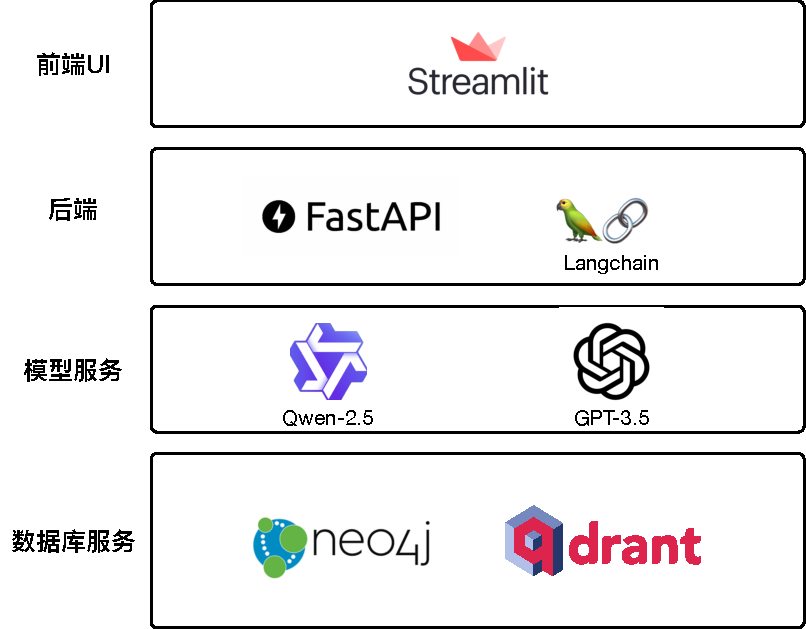
\includegraphics[height=6cm]{../assets/ch5-系统实现图.pdf}
  \bicaption{系统模块图}{System Implementation Diagram}
  \label{fig:implementation}
\end{figure}


\section{本章小结}

本章设计并实现了一个基于知识图谱和大语言模型智能体机制的API编排与调用系统。系统通过集成知识图谱查询、模型管理和向量相似度计算功能,为用户提供自然语言交互的低门槛界面,并支持复杂需求的API调用和回答生成。系统架构分为存储层、访问层、功能层、接口层和展示层,涵盖从数据存储与检索到用户交互的全链路设计。主要功能包括任务分解模块与API动态编排、API调用流程管理、历史调用参考、自定义工具扩展以及多轮问答支持。系统实现采用FastAPI作为后端框架,结合Streamlit前端和Neo4j、Qdrant等数据库,实现了模块化、用户友好、可扩展的交互体验,满足了多样化的用户需求并提供高效的API编排与调用服务。
% !TEX root = ../main.tex

\chapter{总结与展望}

\indent 本章共包括两个部分,第一个部分是对全文工作内容进行总结和回顾,第二个部分就是对本工作的不足和局限性进行探讨,并对未来可能的研究探索方向进行探讨。

\section{工作总结}

本文从大语言模型在复杂任务场景中的应用挑战出发,提出了一套完整的解决方案,包括工具图谱构建、动态工具编排与调用方法,以及系统设计与实现,旨在探索如何通过大语言模型与知识图谱的结合实现高效的工具调用和任务解决方案。具体内容涵盖以下三方面:

\begin{enumerate}
    \item 本文提出了一种基于工具调用路径的工具图谱构建方法,系统性地完成了从数据筛选到图谱验证的全流程。通过提取高质量工具组和调用路径,设计了工具知识图谱的概念模型,以描述工具的层次关系与依赖逻辑,构建了工具图谱。该图谱为复杂任务中的工具选择与规划提供了重要支撑,显著提升了工具调用的准确性和效率。
    \item 为应对工具调用过程中的动态性和复杂依赖关系,本文设计了一种基于知识图谱的动态编排与调用方法。通过任务分解模块将复杂需求拆解为可执行的子任务,并结合深度优先搜索算法在图谱中动态规划工具路径,实现了工具调用的灵活性与精确性。引入记忆机制和自我反思机制,进一步提高了调用过程的稳定性和适应性,为多样化任务需求提供了高效解决方案。
    \item 本文基于知识图谱和大语言模型智能体机制,设计并实现了一个用户友好的API编排与调用系统。系统采用模块化架构,涵盖工具管理、任务规划与执行、以及智能问答功能,为用户提供了低门槛的交互体验。通过自然语言解析需求,系统能够自动完成API调用流程,实现了工具调用的自动化和可视化,展现了高效性与扩展性。
\end{enumerate}

\section{未来展望}

本文围绕着如何构建有效的API工具图谱、并将大量API工具集成到大语言模型中进行了一系列的探索,
然而本文工作仍面临着许多不足之处和可以持续探索的空间。
以下几点是未来可以持续探索和改进的方向。

\indent 1.本文中提出的基于工具调用路径数据构建工具图谱的方法,
在工具图谱的构建过程中,我们只考虑了工具之间的跳转关系,而没有考虑到工具之间的替换关系。
然而在现实工具调用场景中,当一个工具不稳定或者实效时,用户可能
需要选择其他在功能上有替换关系的工具进行代替。
如何在工具图谱中考虑更多的工具之间的关系,并挖掘更丰富的工具关系,是
未来值得探索的方向。

\indent 2.本文中并未对大语言模型进行微调,而是直接使用了训练好的开源模型或GPT-3.5等闭源模型。
但是,大语言模型工具集成的一个重要研究方向就是如何通过微调让模型获得更好的工具调用效果。
现在有许多工作聚焦于微调规模较小的大语言模型,以提升其对工具任务的理解能力和工具方面的规划、推理能力。
经过大规模语料预训练的模型中具有许多工具调用的知识,在未来如何通过有监督的微调来更好挖掘大模型在工具
方面的潜力,并有效提升工具调用的效果,也是下一步需要研究的方向。

\indent 3.为了提升系统的易用性和用户体验,我们可以进一步优化系统的界面设计和
交互设计,使其更加直观和用户友好。同时,本系统仅在少量用户的情况下进行了测试,未来
可以对该系统的性能和稳定性进行持续改进,以确保在大规模用户同时使用的情况下依然能够保持高效
和稳定地提供服务。


%TC:ignore

% 参考文献
\printbibliography[heading=bibintoc]

% 附录
\appendix

% 附录中图表不加入索引
\captionsetup{list=no}

% 附录内容
\input{contents/app_maxwell_equations}
\input{contents/app_flow_chart}

% 结尾部分
\backmatter

% 用于盲审的论文需隐去致谢、发表论文、科研成果、简历

% 致谢
% !TEX root = ../main.tex

\begin{acknowledgements}
 
  研究生时光悄然流逝,转眼间已经到了毕业的时刻。回望这两年多的学习和生活,我不仅学到了知识,更收获了许多关心和帮助。在这个特别的节点,我想真诚地感谢一路上支持和陪伴我的人。
  
  首先,感谢我的导师吴刚老师。从大四开始,吴老师就一直是我的指导老师。在科研方向选择、论文写作、思路调整等方面,吴老师始终耐心地帮助我,为我解答疑惑、指明方向。这让我能够迅速融入交大的校园生活,顺利开启研究生阶段的学习和科研任务。我从吴老师身上学到了科研的严谨态度,也感受到了师者的无私关怀。
  
  感谢我的行业导师赵俊峰老师。赵老师在学术和生活上都给予了我许多帮助,她让我有机会接触到各种工程项目和前沿技术,开阔了视野,也让我对行业有了更深的理解。赵老师的指导让我在实践中成长,是我研究生阶段的一笔重要财富。
  
  感谢我的父母,他们始终是我最坚强的后盾。在求学路上,父母总是默默支持着我,即使对我的研究领域并不熟悉,也从不吝啬鼓励和陪伴。在我遇到挫折和困难时,他们的安慰和理解让我有了重新出发的勇气。我知道,没有他们的支持,就没有今天的我。
  
  感谢南湖实验室。在这两年的联合培养中,实验室为我们提供了良好的科研和生活环境,让我能够专注于学术研究。这一年多的时间不仅让我学到了许多专业知识,也积累了许多美好的回忆。南湖实验室将永远是我研究生生活中最特别的一部分。
  
  感谢我的朋友们,你们让我的研究生生活变得更加丰富和温暖。感谢我的室友李梦瑶同学,尽管我们性格迥异,但我们求同存异,始终彼此支持和帮助。感谢丁鸿馨同学,你的乐观和认真让我倍感鼓舞,认识你是我的幸运。感谢志远、瑞庆、方越师兄,在我遇到学术难题时,你们的耐心解答和宝贵建议为我指明了方向,让我感受到来自实验室的温暖。感谢朱润川同学。你的乐观和热心给身边的人带来了许多正能量。感谢江长江同学,你豁达的人生态度对我有许多启发,我也因你对人生有了不一样的理解,能够更加成熟地面对生活。
  
  最后,我想感谢自己。不管是科研还是实习,这段路并不总是轻松,但我依然坚持到了最后,感谢自己未曾松懈。也感谢自己一直相信自己。
  
  未来,我将带着这些珍贵的回忆与感激之情,继续前行,迎接人生新的篇章。

\end{acknowledgements}


% 发表论文及科研成果
% 盲审论文中,发表论文及科研成果等仅以第几作者注明即可,不要出现作者或他人姓名
% !TEX root = ../main.tex

\begin{achievements}

\subsection*{专利}

\begin{bibliolist}{00}
  \item 第一发明人, “一种基于智能体与知识图谱的任务编排方法与系统”, 专利申请号202411237239.0.
\end{bibliolist}

\end{achievements}


% 学士学位论文要求在最后有一个大摘要,单独编页码
\input{contents/digest}

%TC:endignore

\end{document}
